%!TEX program = xelatex
% 完整编译: xelatex -> bibtex -> xelatex -> xelatex
\documentclass[lang=cn,11pt,a4paper,cite=authoryear]{elegantpaper}


\title{文献分享——Prediction, Estimation, and Attribution}
\author{Author: Bradley Efron,\quad 分享人:史宏炜}
%\institute{\href{https://elegantlatex.org/}{Elegant\LaTeX{} 项目组}}
%
%\version{0.09}
\date{\zhtoday}


% 本文档命令
\usepackage{array}
\usepackage{subfigure}
\usepackage{float}
\usepackage{multirow} % 跨行排列
\usepackage{rotating} % 宽表格
\newcommand{\ccr}[1]{\makecell{{\color{#1}\rule{1cm}{1cm}}}}

% 参考文献上标
\newcommand{\upcite}[1]{\textsuperscript{\textsuperscript{\cite{#1}}}}
% 修改参考文献名字
\renewcommand\refname{References}

% 添加英文摘要
\newcommand{\ekeywords}[1]{\vskip2ex\par\noindent\normalfont{\bfseries Key Words: }#1}

% 罗马数字
\newcommand{\RNum}[1]{\uppercase\expandafter{\romannumeral #1\relax}}

% 修改编号方式
%\renewcommand {\thefigure} {\thesection{}-\arabic{figure}}
%\renewcommand {\thetable} {\thesection{}-\arabic{table}}
%\numberwithin{equation}{section}

%----------------------------------------------------------------
%想把特定符号的定义从fysymbol宏包里抽出来,以和amsfonts、amssymb保持兼容
\makeatletter
% for explaination, see `texdoc fntguide`
% excerpted from `fdsymbol.sty`
\newcommand{\fdsy@scale}{1.0}
\newcommand\fdsy@mweight@normal{Book}
\newcommand\fdsy@mweight@small{Book}
\newcommand\fdsy@bweight@normal{Medium}
\newcommand\fdsy@bweight@small{Medium}
\DeclareFontFamily{U}{FdSymbolC}{}
\DeclareFontShape{U}{FdSymbolC}{m}{n}{
    <-7.1> s * [\fdsy@scale] FdSymbolC-\fdsy@mweight@small
    <7.1-> s * [\fdsy@scale] FdSymbolC-\fdsy@mweight@normal
}{}
\DeclareFontShape{U}{FdSymbolC}{b}{n}{
    <-7.1> s * [\fdsy@scale] FdSymbolC-\fdsy@bweight@small
    <7.1-> s * [\fdsy@scale] FdSymbolC-\fdsy@bweight@normal
}{}
\DeclareSymbolFont{arrows}{U}{FdSymbolC}{m}{n}
\SetSymbolFont{arrows}{bold}{U}{FdSymbolC}{b}{n}
% use \DeclareMathSymbol directly
\DeclareMathSymbol{\upvDash}{\mathrel}{arrows}{233}
\let\Vbar\upvDash
\DeclareMathSymbol{\upmodels}{\mathrel}{arrows}{237}
\makeatother
%----------------------------------------------------------------

\begin{document}

\maketitle

Prediction, Estimation, and Attribution是统计学家Bradley Efron于2020年发表在International Statistical Review的一篇综述。

20世纪的科学需求和计算方面的限制塑造了传统的统计方法论,但在21世纪,需求和限制都有所改变,方法论也相应地发生了变化。大规模的预测算法——神经网络、深度学习、boosting、支持向量机、随机森林等已经在主流媒体上获得了明星的地位。他们被视作传统回归方法的继承者,可以在巨大规模的数据集上运行。学者Efron在这篇综述中总结了传统回归方法(traditional regression methods)和纯预测算法(pure prediction algorithms)之间的主要区别,主要集中在prediction和estimation之间以及prediction和attribution (significance testing)之间,文章中的大部分讨论是通过一些比较小的数值例子展示的。通过阐述传统回归方法和预测算法具有的优势以及不足,Efron提出了对传统回归方法以及预测算法未来发展的两个期待,指出了我们有将传统方法论和现代算法相结合并继续探索新方法的可能性:
\begin{enumerate}
	\item 希望预测算法的输出结果更具可解释性(\textcolor{blue}{Trend 1 aims to make the output of a prediction algorithm more interpretable})。
	\item 希望在传统方法论的框架内,至少能够实现一些预测算法所具有的优点(\textcolor{blue}{Trend 2 hopes to achieve at least some of the advantages of prediction algorithms within a traditional framework})。
\end{enumerate}

\section{Introduction}

统计回归方法要追溯到19世纪初的高斯(Gauss)和勒让德(Legendre),特别是1877年的高尔顿(Galton)时期。在19世纪期间,回归的思想适用于大多数重要的统计任务:新案例的预测、回归表面(regression surfaces)的估计以及对单个预测变量的重要性进行评估(在文章的标题中称作"attribution")等。在20世纪,很多有力的统计思想都和回归有千丝万缕联系:最小二乘拟合、逻辑回归、广义线性模型、ANOVA、预测变量显著性检验和均值回归等。

21世纪见证了一种新型的“纯预测算法”(pure prediction algorithms)的崛起——神经网络、深度学习、boosting、支持向量机和随机森林,这些算法和Guass-Galton的传统方法有明显的区别,而且它们可以在拥有数百万个数据点和甚至更多的预测变量的巨大规模数据集上运行。这些算法(尤其是深度学习)在自动化任务方面非常成功,如在线购物、机器翻译和航线信息(airline information),他们凭借自身的优势成为了媒体的宠儿,也引发了商业界的巨大兴趣。最近这股热潮已经扩散到了科学界,在浏览器中马上就可以检索到“生物学上的深度学习”(deep learning in biology)、“计算语言学与深度学习”(computational linguistics and deep learning)、“调节基因组学的深度学习”(deep learning for regulatory genomics)等相关词条。

纯预测算法如何与传统的回归方法相关联(\textcolor{blue}{How do the pure prediction algorithms relate to traditional regression methods?}),是Efron在这篇综述中要探讨的中心问题。一系列显著的差异将在综述中被验证——假设方面、科学理念以及目标方面的差异。讲清楚这件事是很复杂的,两者也并没有清晰的胜负之分。Efron给出了一个粗略的总结:纯预测算法为统计学家的“军械库”增添了强大的力量,但其常规的科学适用性还需要进一步的发展(\textcolor{blue}{the pure prediction algorithms are a powerful addition to the statistician's armory, yet substantial further development is needed for their routine scientific applicability})。而且这样的发展已经在统计学的世界中进行了,并为我们的学科提供了可喜的能量和活力。

Efron的这篇综述,最初是一个报告(talk presentation can download in \href{http://statweb.stanford.edu/~ckirby/brad/talks/2019Predict-Estimat-Attribut.pdf}{2019Predict-Estimat-Attribut.pdf}),是用一种宽泛的笔触写成的,旨在描述当前的实践,而不是强调事情必须是怎样的。

Efron在文章中写道:这不是一篇研究性的论文,大部分的论证都是通过数值的例子进行的。这些例子的规模很小,以目前的预测标准来衡量甚至是不值一提的。某种“巨型主义”已经占据了预测类的文献,带有一些膨胀的前缀,如tera-, peta-。但是小的数据集可以更好地暴露出新方法的局限性。\cite{hastie2009elements}是有关预测方法的一个很好的参考,无论是传统的还是现代的方法。

\section{Surface Plus Noise Models}

对于预测算法和传统的回归方法,文中假设数据集$\bold{d}$具有以下结构:
\begin{align}
\label{data}
	\bold{d}=\left\{\left(x_{i}, y_{i}\right), i=1,2, \ldots, n\right\}
\end{align}
其中$x_i$是$p$维的预测变量,$x_i$来自一个已知空间$\mathcal{X}$,$\mathcal{X} \subset \mathbb{R}^p$,$y_i$是一个真值响应变量。假设$n$对数据是相互独立的,更简化的形式可以写为:
\begin{align}
	\bold{d}=\{\bold{x}, \bold{y}\}
\end{align}
其中$\bold{x}$是$n \times p$的矩阵,$\bold{y} = (y_1, y_2, \ldots , y_n)^t$。假定最传统回归模型如下:
\begin{align}
\label{regression model}
y_{i}=x_{i}^{t} \beta+\epsilon_{i} \quad(i=1,2, \ldots, n)
\end{align}
其中$\epsilon_{i} \stackrel{\text { iid }}{\sim} \mathcal{N}\left(0, \sigma^{2}\right)$,$\beta$是一个$p$维的未知参数向量。以矩阵的形式可以写为:
\begin{align}
\bold{y}=\bold{x} \beta+\epsilon
\end{align}

对任意的$x \in \mathcal{X}$,模型(\ref{regression model})中响应变量$y$的期望为$\mu = x^t \beta$,因此$y \sim N(\mu, \sigma^2)$。线性表面(linear surface)可以表示为:
\begin{align}
\mathcal{S}_{\beta}=\left\{\mu=x^{t} \beta, x \in \mathcal{X}\right\}
\end{align}
surface中包含着所有真实的期望,但是真正的事实会被噪声项$\epsilon_i$所模糊。

更一般的情况,可以将模型(\ref{regression model})扩展为:
\begin{align}
\label{general regression model}
y_{i}=s(x_i, \beta)+\epsilon_{i} \quad(i=1,2, \ldots, n)
\end{align}
其中$s(x, \beta)$是某个已知的函数形式,对于任意固定的$\beta$,所得$\mu = s(x, \beta)$是一个关于$x \in \mathcal{X}$的函数。真实的期望表面,也就是回归表面(regression surface)表示为:
\begin{align}
\mathcal{S}_{\beta}=\left\{\mu=s(x, \beta), x \in \mathcal{X}\right\}
\end{align}

大多数传统的回归模型依赖于某种“表面加噪声”(\textcolor{blue}{surface plus noise})的公式。surface描述的是我们希望学习到的科学真理,但我们只能观察surface上被噪声掩盖的点。统计学家的传统估计任务就是是从数据$\bold{d}$中尽可能多地学习到surface。

\subsection{Example 1}

文中通过一个小的例子来展示surface plus noise模型,数据集是从\cite{efron1991compliance}的大数据集中提取的:$n=164$名男性医生自愿服用降胆固醇药物cholostyramine。对于每个医生记录以下两组数据:
\begin{align}
\begin{array}{l}
x_{i}=\text { normalized compliance } \quad \text { and } \\
y_{i}=\text { observed cholesterol decrease. }
\end{array}
\end{align}

Compliance (依从性)是指某个受试者实际服用的剂量占计划剂量的比例,范围从0\%到100\%,正态化之后是从-2.25到1.97。希望看到依从性越好,胆固醇降低的越多。

利用这组数据拟合了模型(\ref{general regression model}),$s\left(x_{i}, \beta\right)$具有以下形式:
\begin{align}
s\left(x_{i}, \beta\right)=\beta_{0}+\beta_{1} x_{i}+\beta_{2} x_{i}^{2}+\beta_{3} x_{i}^{3}
\end{align}
也就是说这是一个三次回归模型,拟合结果如图(\ref{fig1})所展示(\textcolor{blue}{附件中提供了所有例子的R code})。
\begin{figure}[H]
		\centering
		\subfigure[Efron's article]{
			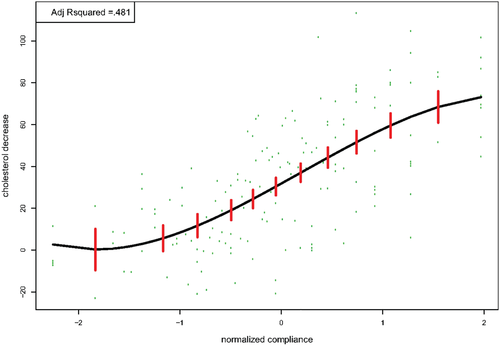
\includegraphics[width=6.5cm]{Fig1.png}
		}\\
		\subfigure[Replot (Method 1)]{
			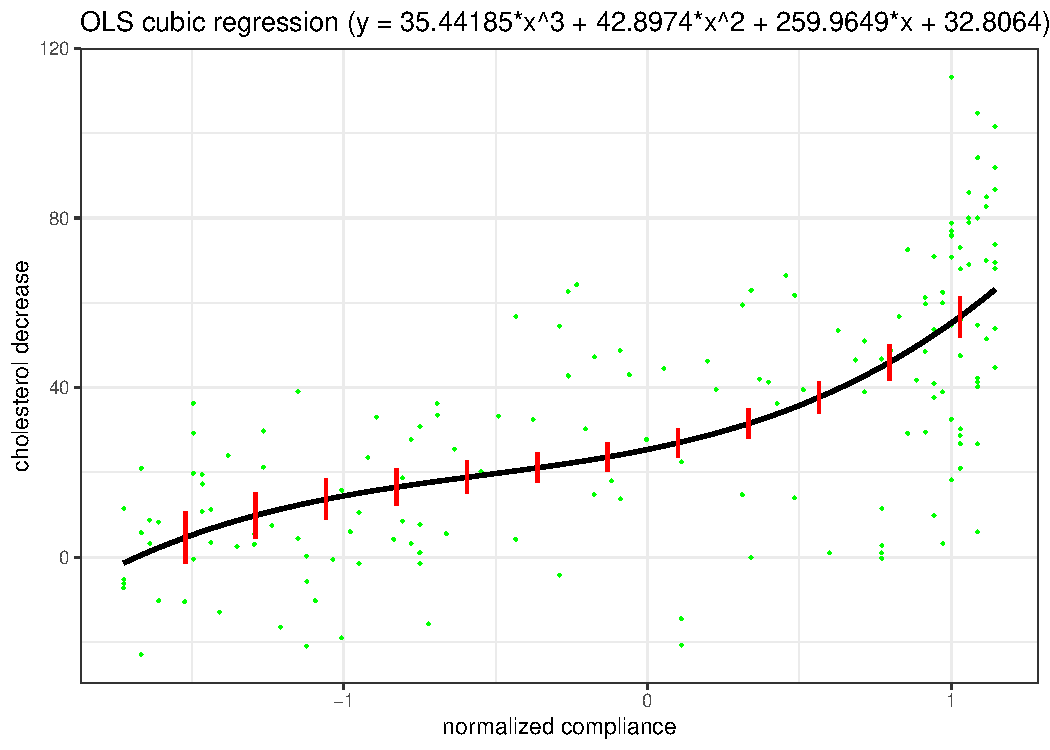
\includegraphics[width=6.5cm]{fig1.pdf}
		}
		\subfigure[Replot (Method 2)]{
			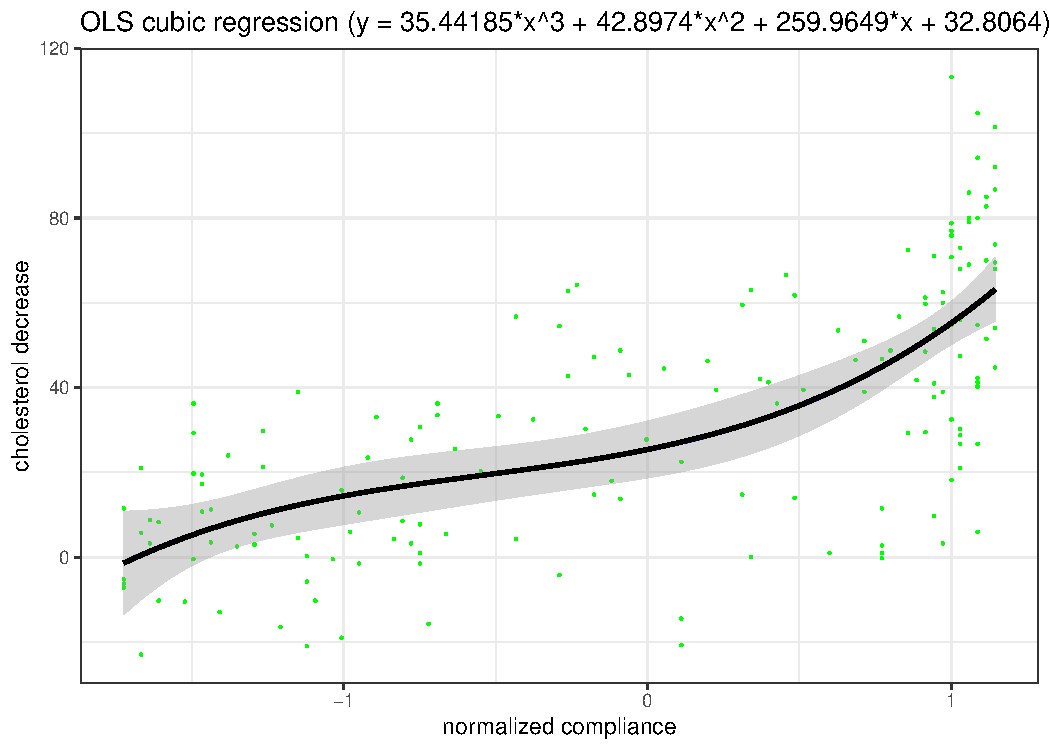
\includegraphics[width=6.5cm]{fig1_.pdf}
		}
		\caption{Black curve is OLS fitted regression to cholostyramine data (dots); vertical bars indicate $\pm$ one standard error estimation}
		\label{fig1}
\end{figure}

图(\ref{fig1})中黑色的曲线表示估计的surface:
\begin{align}
	\widehat{\mathcal{S}} = \{s(x, \widehat{\beta}) \quad \text{for} \quad x \in \mathcal{X}) \}
\end{align}
这是通过极大似然的方法拟合的,也等价为通过最小二乘(OLS)方法拟合的。垂直的竖线表示估计值$s(x, \widehat{\beta})$加减一个标准误,为了表示用$\widehat{\mathcal{S}}$来估计真实的$\mathcal{S}$的不准确程度。

以上讲述的是estimation方面的内容。就attribution而言,只有$\widehat{\beta}_0$和$\widehat{\beta}_1$是显著非零的,调整的$R^2$为0.482,$R^2$是模型预测能力的一种传统度量。

另外一个传统研究方法的中流砥柱是逻辑回归,表(\ref{table1})考虑了一组新生儿数据(neonate data):在非洲的工厂中,$n=812$个生病的新生儿经历了长达一年的观察,其中605个活着,207个死亡。neonate data记录了11个协变量,$y_i$为0或1用来表示新生儿是死亡还是或者。这是一个具有线性对数的surface以及bernoulli noise的surface plus noise模型。
\begin{table}[H]
    \centering
    \caption{Logistic regression analysis of neonate data}
    \label{table1}
    \begin{tabular}{lcll}
    	\toprule
         & Estimate & SE & $p$-value \\ 
        \midrule
        Intercept & –1.549 & 0.457 & 0.001*** \\ 
        gest & –0.474 & 0.163 & 0.004** \\ 
        ap & –0.583 & 0.110 & 0.000*** \\ 
        bwei & –0.488 & 0.163 & 0.003** \\ 
        resp & 0.784 & 0.140 & 0.000*** \\ 
        cpap & 0.271 & 0.122 & 0.027* \\ 
        ment & 1.105 & 0.271 & 0.000*** \\ 
        rate & –0.089 & 0.176 & 0.612 \\ 
        hr & 0.013 & 0.108 & 0.905 \\ 
        head & 0.103 & 0.111 & 0.355 \\ 
        gen & –0.001 & 0.109 & 0.994 \\ 
        temp & 0.015 & 0.124 & 0.905 \\ 
        \bottomrule
    \end{tabular}
\end{table}

将11个预测变量标准化,使其均值为0,方差为1,然后进行逻辑回归分析。表(\ref{table1})展示了一些输出结果。第1列和第2列给出了回归系数的估计和标准误。第3列展示了11个变量的双边$p$值,其中6个变量显著非零,这就是分析的attribution部分。就prediction而言,拟合逻辑回归模型给出了每个婴儿的死亡概率$p_i$的估计值。预测规则为:
\begin{align}
\begin{array}{l}
\text{if}\quad p_i > 0.25 \qquad \text{predict \qquad dies} \\
\text{if}\quad p_i \leq 0.25 \qquad \text{predict \qquad lives}
\end{array}
\end{align}
得到的经验误差率为18\%。

\subsection{Example 2}
真理的诞生往往需要大量的实验,不要以为牛顿第二定律完全是牛顿一拍脑袋想象出来的,其实牛顿是一位实验大师,图(\ref{fig2})的左边展示了牛顿第二定律的surface的表现,右边是一幅想象出来的实验数据可能的样子。
\begin{figure}[H]
		\centering
		\subfigure[Efron's article]{
			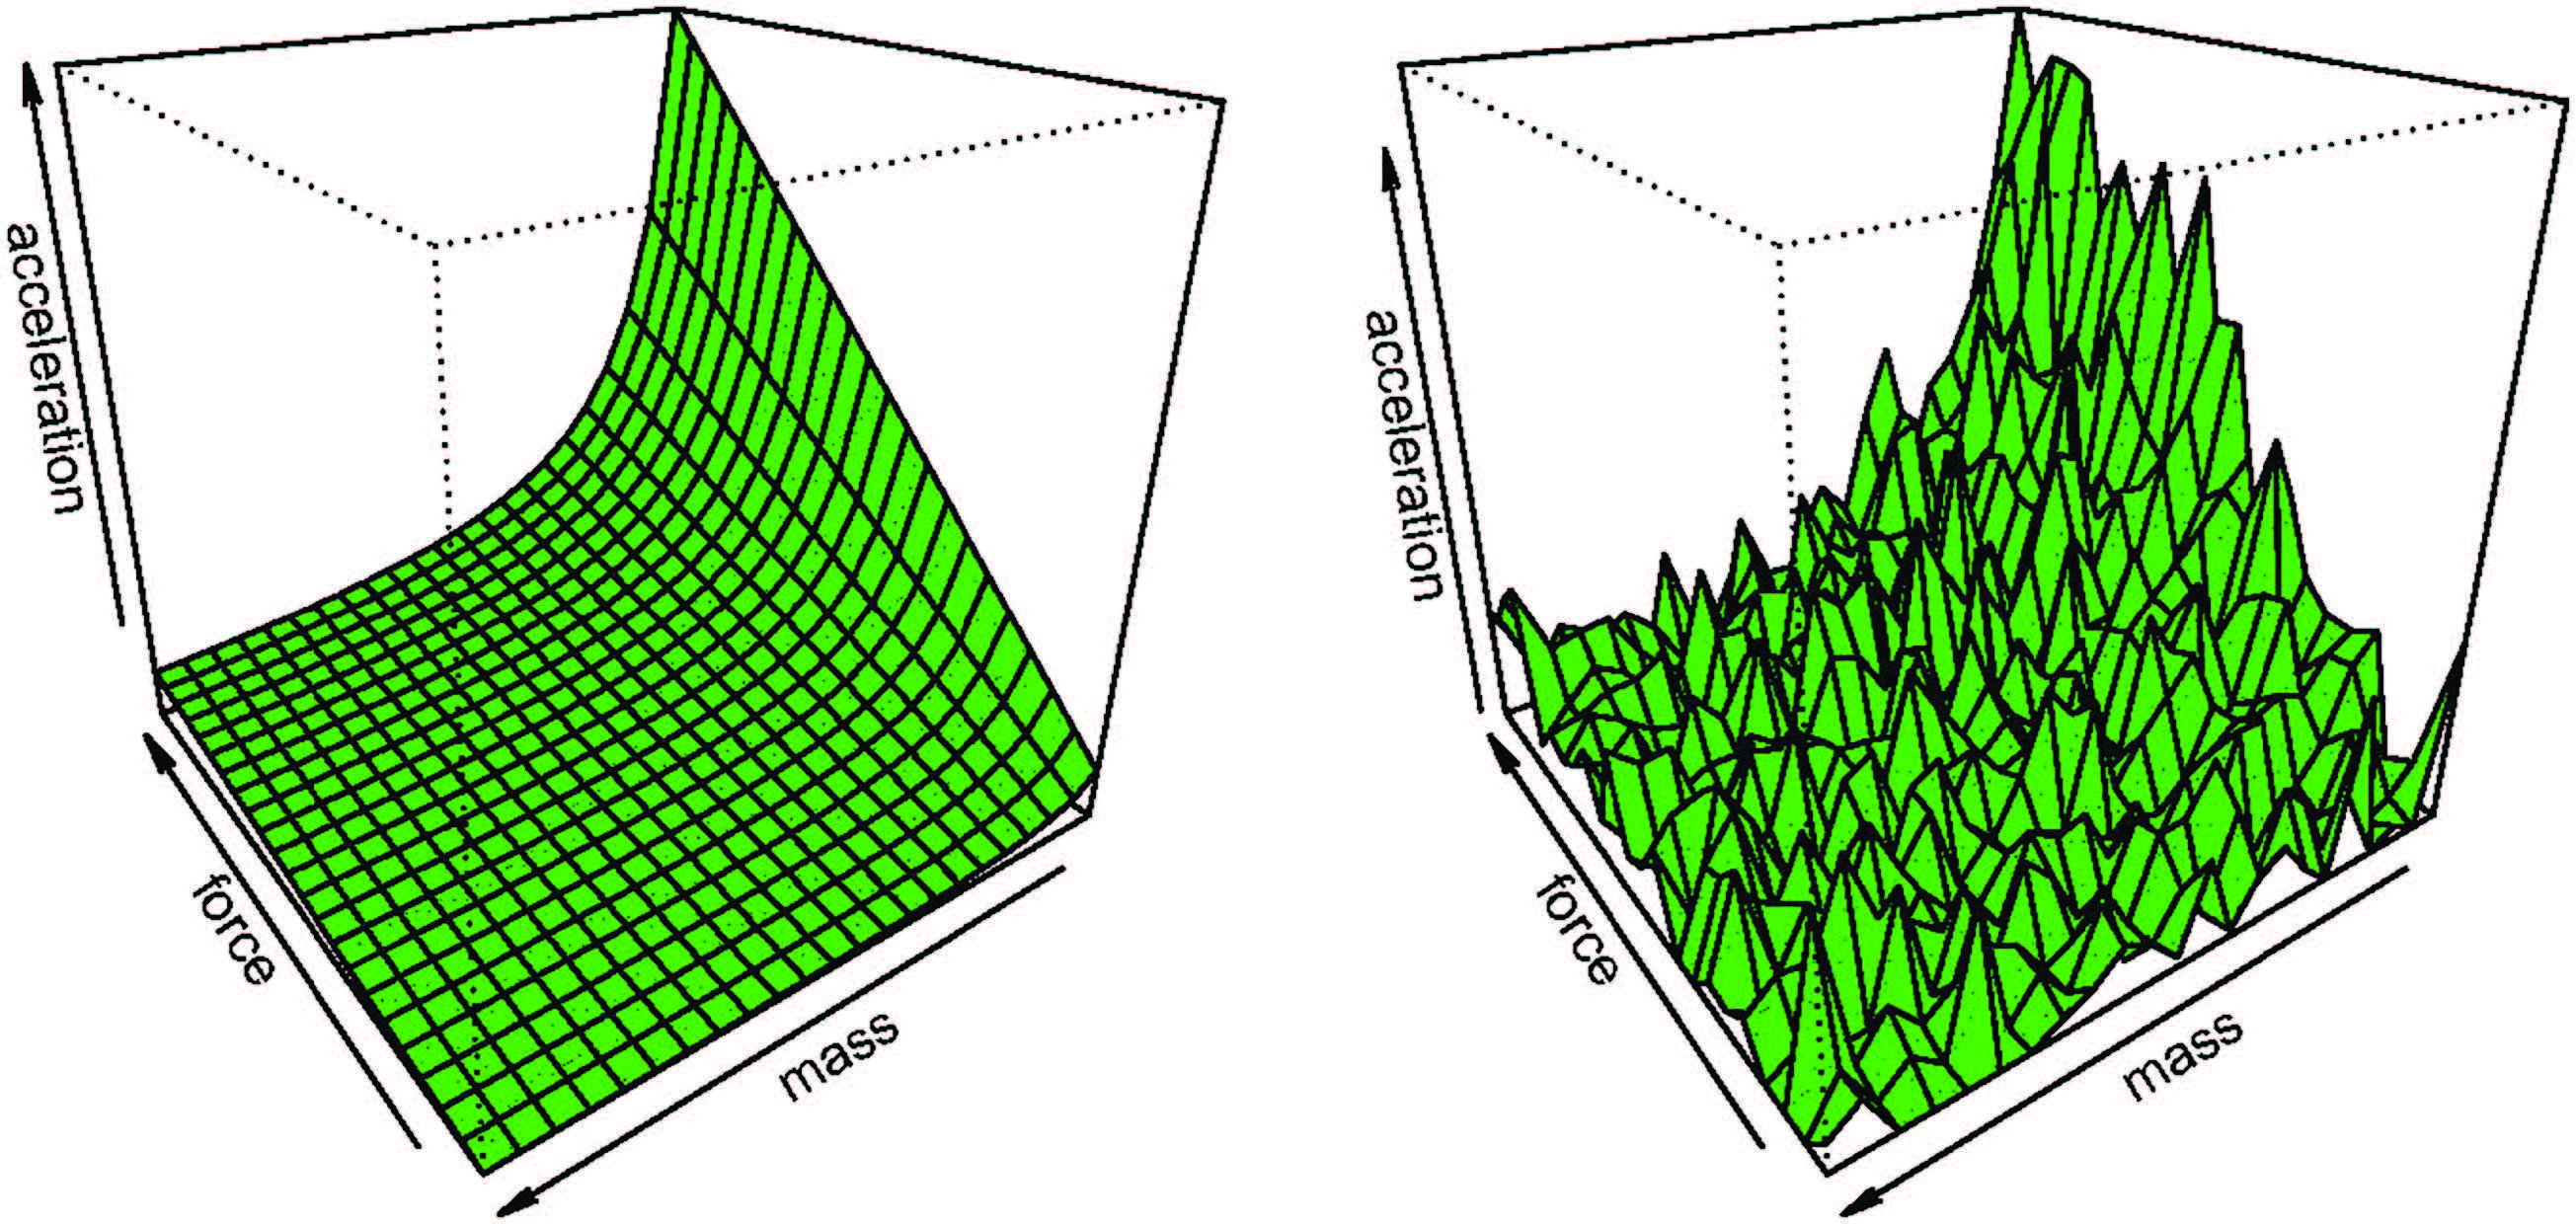
\includegraphics[width=\textwidth]{Fig2.jpg}
		}\\
		\subfigure[Replot]{
			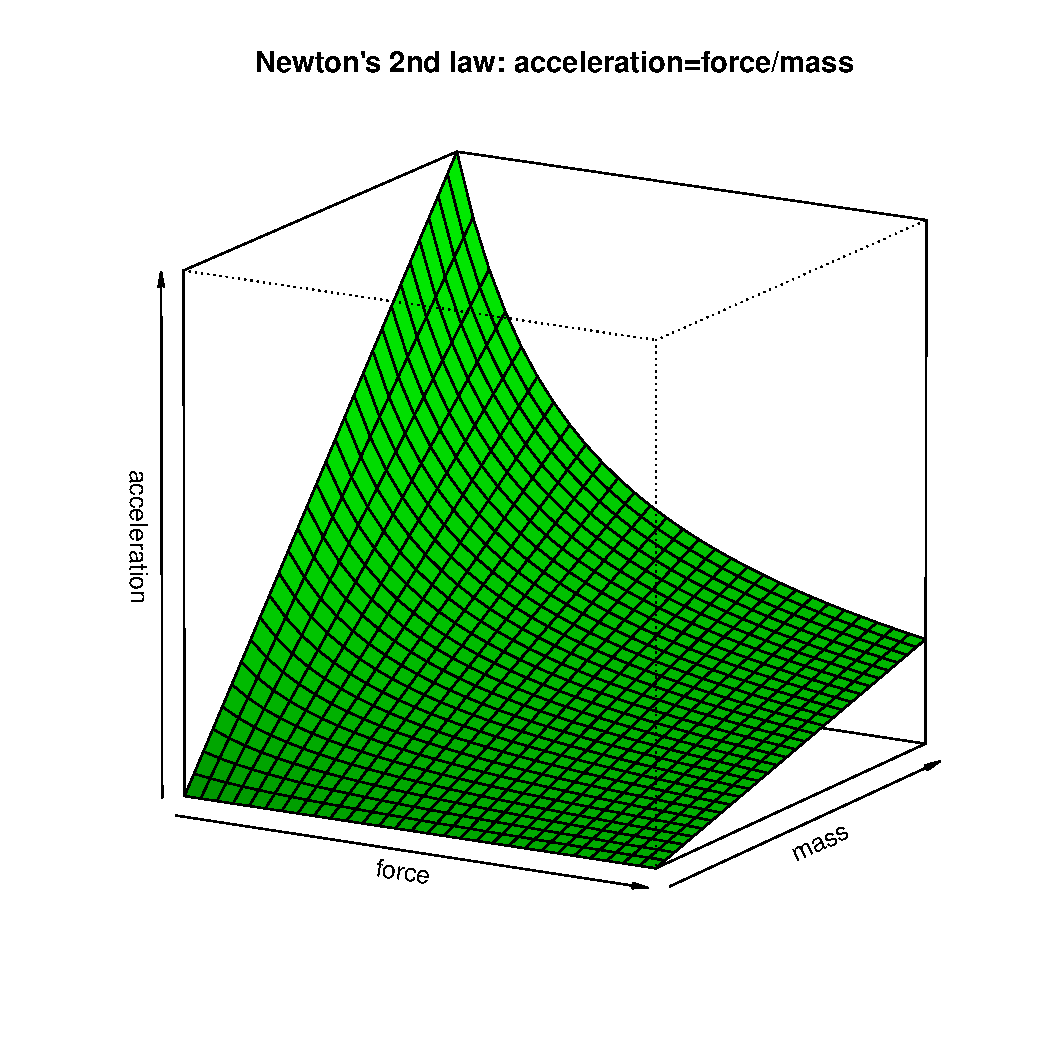
\includegraphics[width=7.7cm]{fig21.pdf}
		}
		\subfigure[Replot]{
			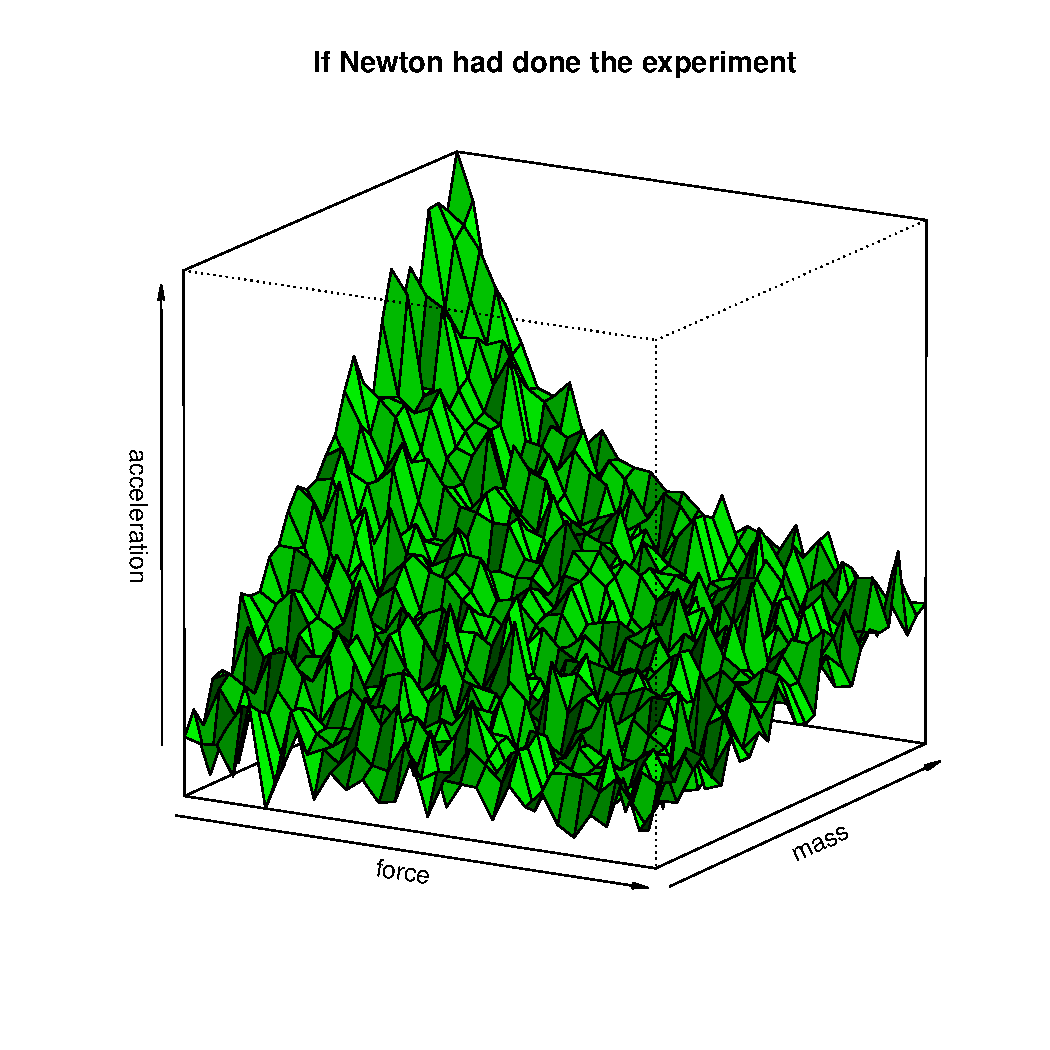
\includegraphics[width=7.7cm]{fig22.pdf}
		}
		\caption{On left, a surface depicting Newton's second law of motion, acceleration=force/mass; on right, a noisy version.}
		\label{fig2}
\end{figure}

在缺乏天才般的洞察力的情况下,统计估计理论旨在作为一种工具,从嘈杂的数据中窥视并识别出平滑的潜在真相。cholostyramine和neonate的例子都不像牛顿第二定律那么根本(fundamental),但它们的共同目标是在嘈杂的环境中提取可靠的科学结构(\textcolor{blue}{they share the goal of extracting dependable scientific structure in a noisy environment})。噪声是短暂的,但结构是永恒的,或至少持久的(\textcolor{blue}{The noise is ephemeral but the structure, hopefully, is eternal, or at least long-lasting})。

\section{The Pure Prediction Algorithms}

21世纪见证了一系列不同寻常的预测算法的发展:随机森林、梯度提升、支持向量机、神经网络(包括深度学习)等。为了区别于上一节介绍的传统预测方法,我将把这些统称为纯预测算法。纯预测算法已经在多个方面取得了惊人的成绩,并引起了公众极大的兴趣,如:机器翻译、iPhone的Siri、面部识别、国际象棋和围棋等方面。如果媒体关注是合适的度量标准,那么纯预测算法就是我们这个时代的统计明星。

之所以使用形容词"pure",是因为预测算法的目标是prediction,在estimation和attribution方面基本上可以忽略不计。他们的基本策略很简单:直接是为了获得高的预测准确度,而不考虑surface plus noise模型(\textcolor{blue}{Their basic strategy is simple: to go directly for high predictive accuracy and not worry about surface plus noise models})。纯预测算法具有一些突出的优势,也有一些缺点。

预测算法的通用程序是:输入一个数据集$\bold{d}$,输出一个准则$f(x, \bold{d})$,利用这个准则,对于任意的预测变量$x$可以得到一个预测值
\begin{align}
	\widehat{y} = f(x, \bold{d})
\end{align}

我们希望表面的错误率(apparent error rate)是小的,对于分类问题错误率具有以下形式:
\begin{align}
\widehat{\text{err}}=\#\left\{f\left(x_{i}, \bold{d}\right) \neq y_{i}\right\} / n
\end{align}
更重要的是,希望真正的错误率(true error rate)也是小的:
\begin{align}
\text{Err}=E\{f(X, \bold{d}) \neq Y\}
\end{align}
其中$(X, Y)$是从给定数据集$\bold{d}$中的$(x_i, y_i)$的概率分布中随机提取得到的。随机森林、boosting、深度学习等算法都以能在复杂情况下得到较小的Err而得名。

纯预测算法除了和传统的预测方法有很大的不同以外,这些算法之间也存在着很大的差异。最容易去描述的算法是随机森林(random forests) (\cite{breiman2001statistical})。对于二分类预测问题,就像neonate data,随机森林的预测结果依赖于分类树(classification tree)的总效果。

\subsection{Example 3}

首先对neonate数据采用单个分类树进行预测,如图(\ref{fig3})所示:
\begin{figure}[H]
		\centering
		\subfigure[Efron's article]{
			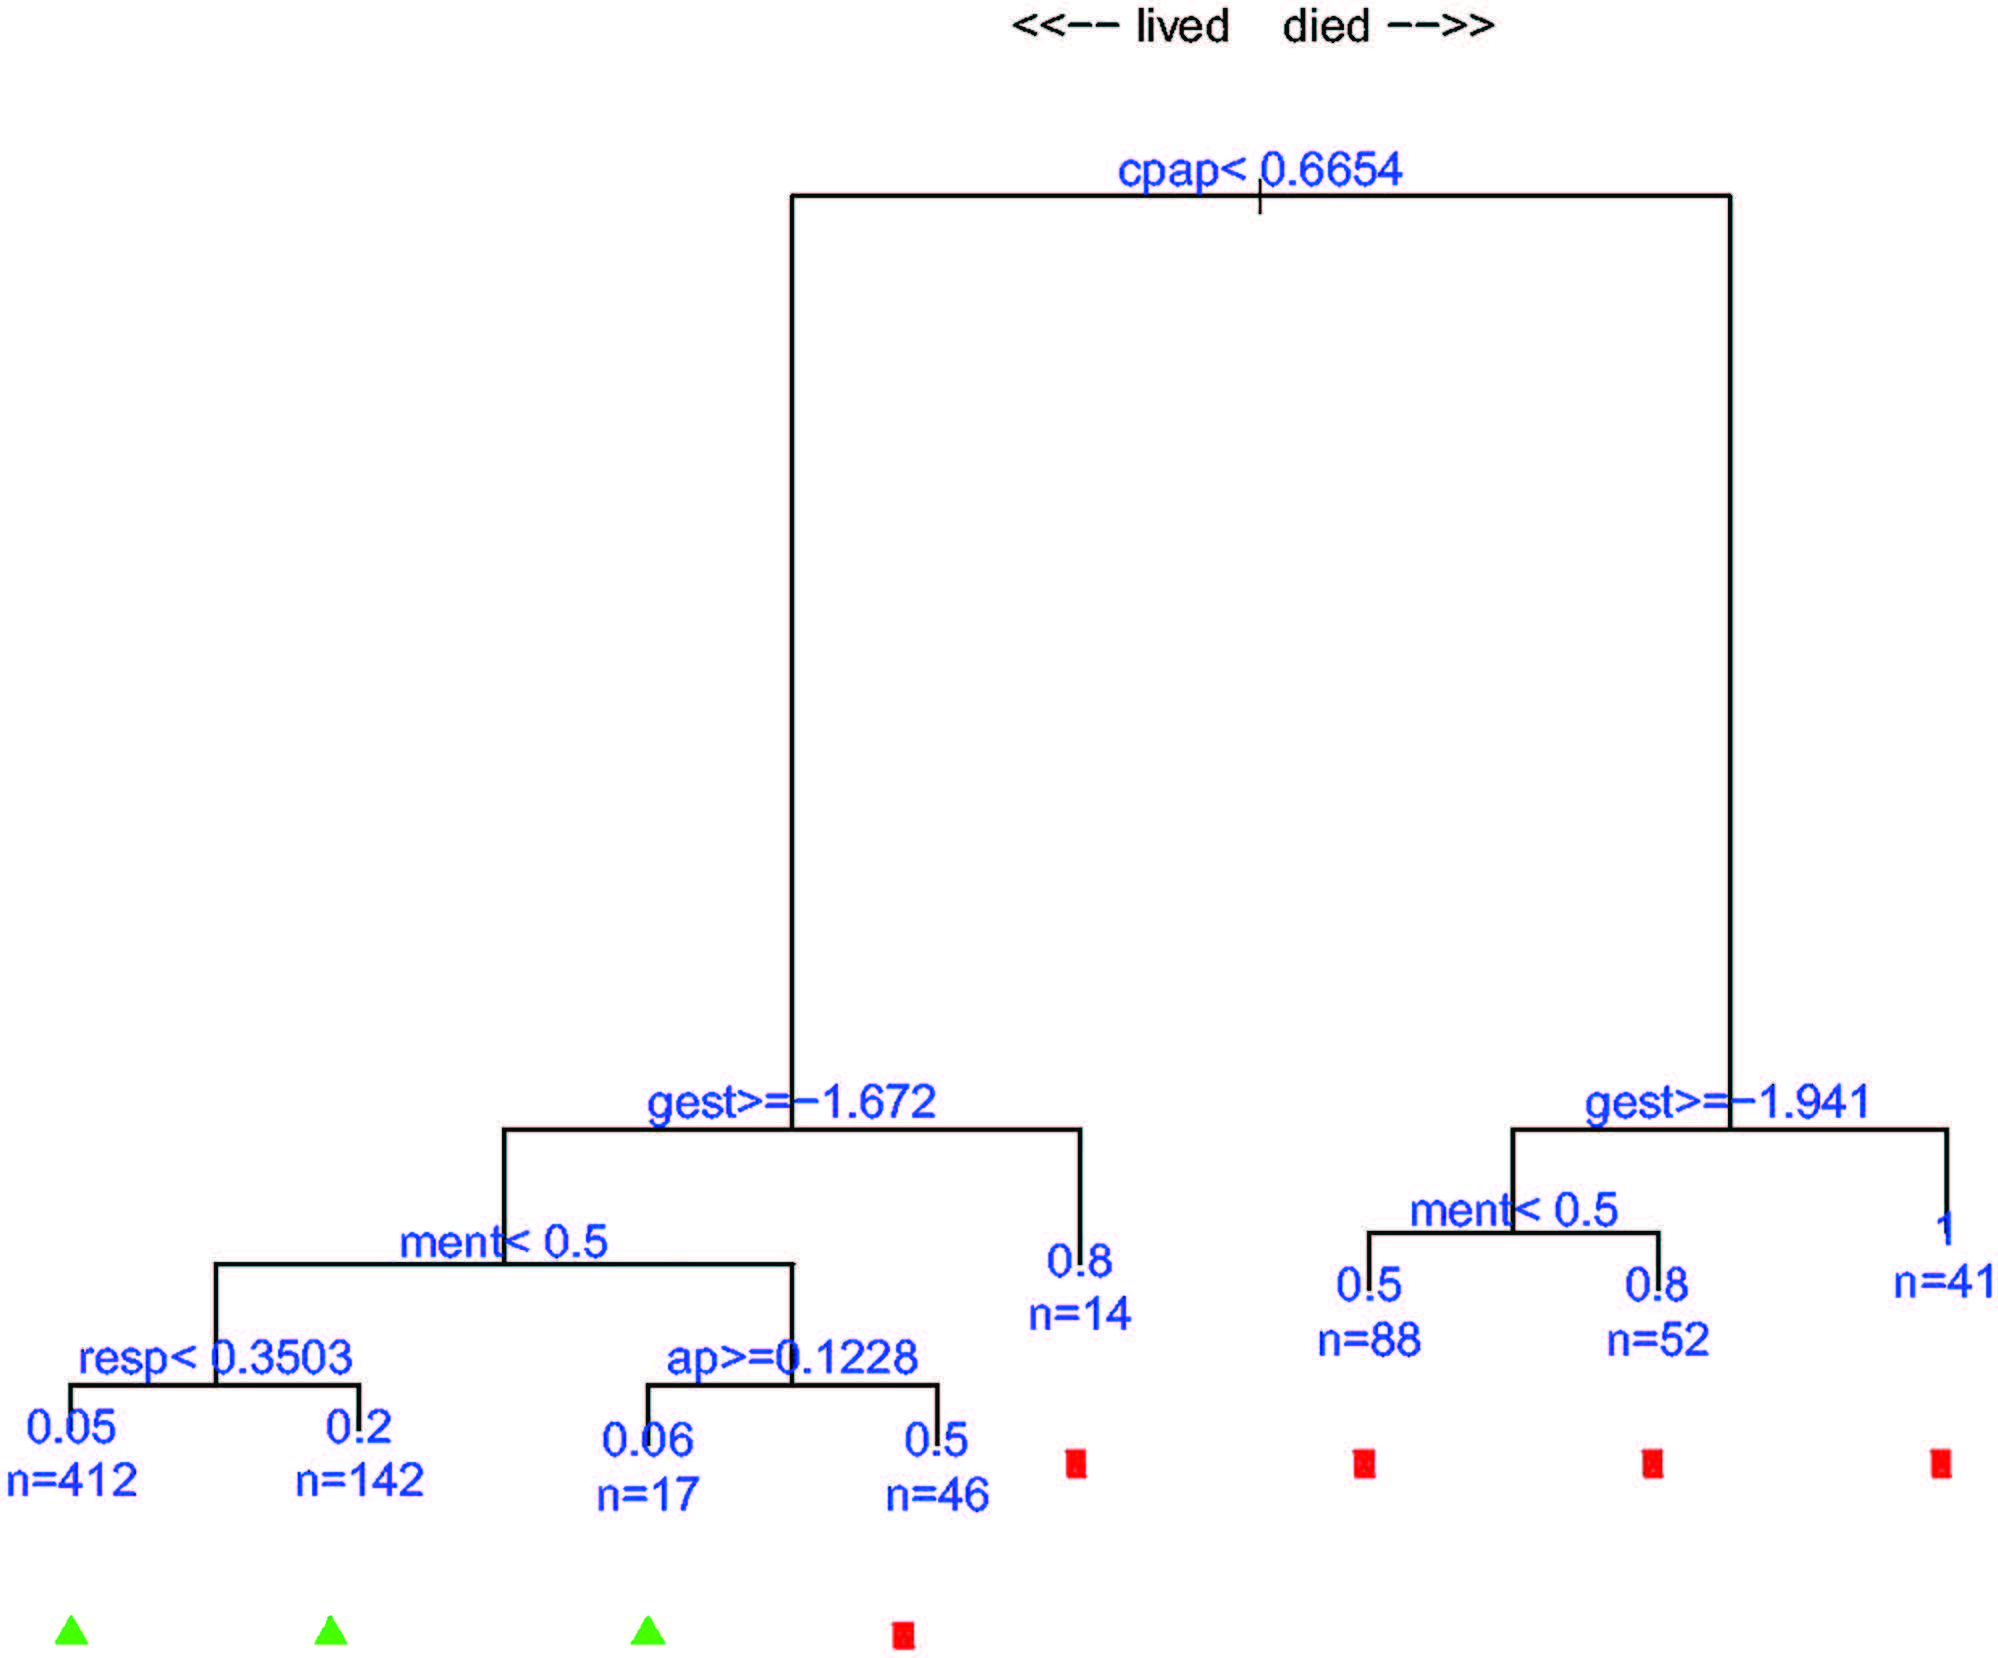
\includegraphics[width=7.7cm]{Fig3.jpg}
		}
		\subfigure[Replot]{
			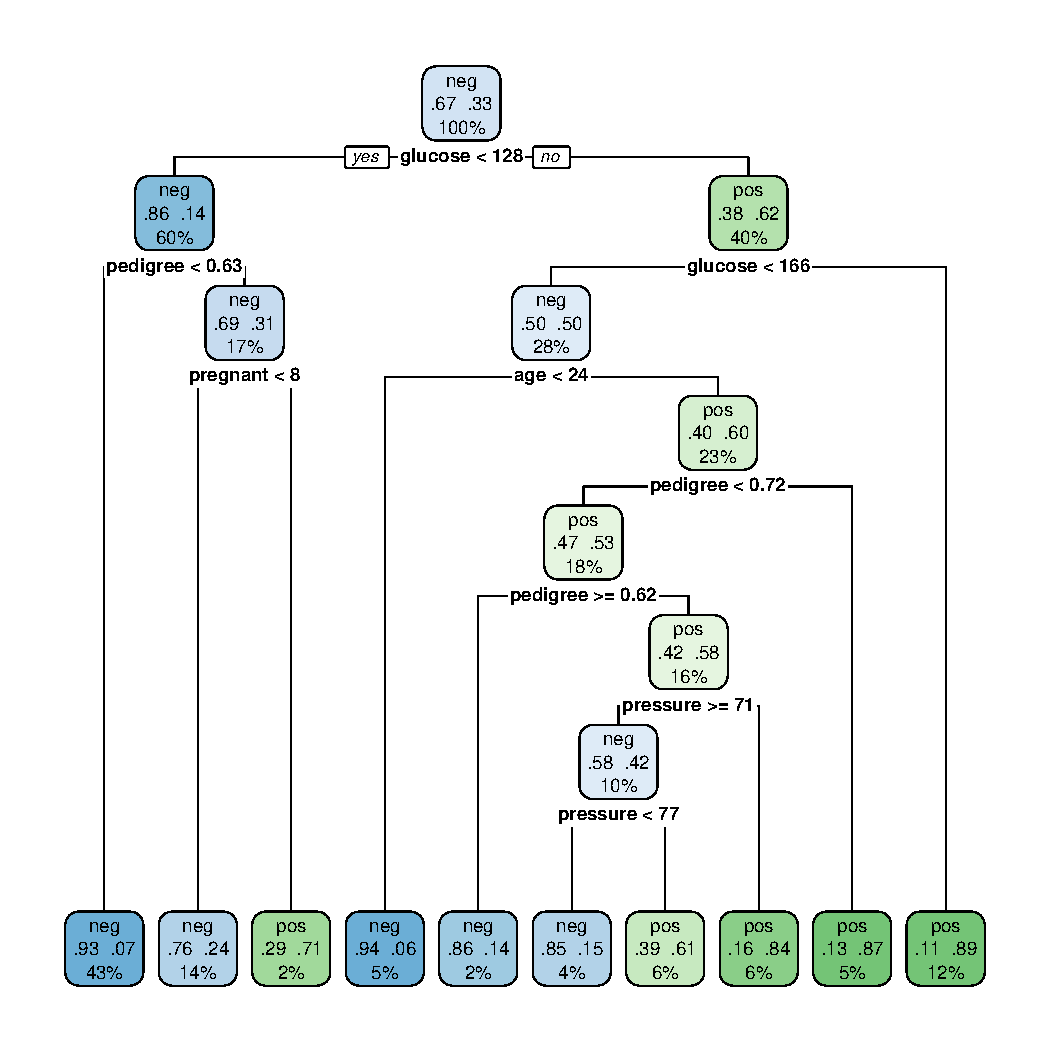
\includegraphics[width=7.7cm]{fig3.pdf}
		}
		\caption{Classification tree for neonate data. Triangled terminal nodes predict baby lives, circled predict baby dies; the rule has apparent prediction error rate 17\% and cross-validated rate 18\%.}
		\label{fig3}
\end{figure}

\noindent{\textbf{注}:由于未能找到neonate data的原始数据集,因此复现时采用了PimaIndiansDiabetes数据集,复现的具体输出结果可以从Rcode中找到。}

从图(\ref{fig3})中可以看出:在树的顶端,812个新生儿被分为两组,选择预测变量cpap和阈值0.6654是为了在所有可能的选择(预测变量、阈值)中最大限度地提高在两个组中死亡率的差异。接着按照相同的Gini系数标准,把两组各自再分为两组。分割过程将一直进行,直到触发了某些停止规则。在图(\ref{fig3})的底端可以看到分割过程以8个终端结点结束:最左边的结点包含了最初812个新生儿中的412个,只有5\%是死亡的;最右侧结点有41名新生儿,全部死亡。三角形表示死亡比例小于原来25.5\%的三个终端结点,方块表示死亡比例超过25.5\%的终端结点。预测规则是:三角形处表示活着,方块处表示死亡。如果有一个新生儿带着具有11个测量值的向量$x$来到医院,医生可以根据$x$的取值沿着分类树从上到下来预测新生儿的生死。

分类树应用到neonate data上所得的预测错误率为17\%,分类树被认为是贪婪的过拟合者,但在这种情况下,10折交叉验证分析给出的错误率为18\%,两者几乎相同。\cite{mediratta2020derivation}对新生儿数据进行了传统的分析,得到了20\%的交叉验证错误率。值得一提的是,在图(\ref{fig3})中的分割变量和表(\ref{table1})中的显著性变量非常吻合。

\subsection{Example 4}

到目前为止,回归树(regression trees)的表现还不错,但在一些更大的例子中,回归树的预测表现很差,见\cite{breiman2001statistical}的Section 9.2。作为一种改进,Breiman 提出的random forest算法依赖于对大量bootstrap trees进行平均,每棵生成的方法如下:
\begin{enumerate}
	\item 从原始数据$\bold{d}$中提取一个非参数的bootstrap样本$\bold{d}^{*}$,即从$\bold{d}$中有放回地抽取$n$对$(x_i, y_i)$的随机样本。
	\item 像之前一样,利用样本$\bold{d}^{*}$构建一个分类树,但仅从$p^{*}$中来选择每次分割,$p^{*}$是在原始的$p$个预测变量中独立地选择出的随机预测变量子集。
\end{enumerate}

生成$B$个这样的分类树之后,一个新的观测$x$在每棵树上得到一个分类结果,最终$\widehat{y} = f(x, \bold{d})$是由$B$中的大多数分类结果决定的。通常$B$取值范围为100-1000。

对neonate data应用random forest的方法进行预测,结果如图(\ref{fig4})。预测错误率表示为一个关于bootstrap trees的数量的函数。总的来说,使用了$B=501$棵树,但在200之后预测错误率的变化不大。总体预测错误率在17\%左右波动,与图(\ref{fig3})中18\%的交叉验证错误率相比只有一点点改进。在第4节的微阵列例子中,random forest显示出了更好的优势。
\begin{figure}[H]
		\centering
		\subfigure[Efron's article]{
			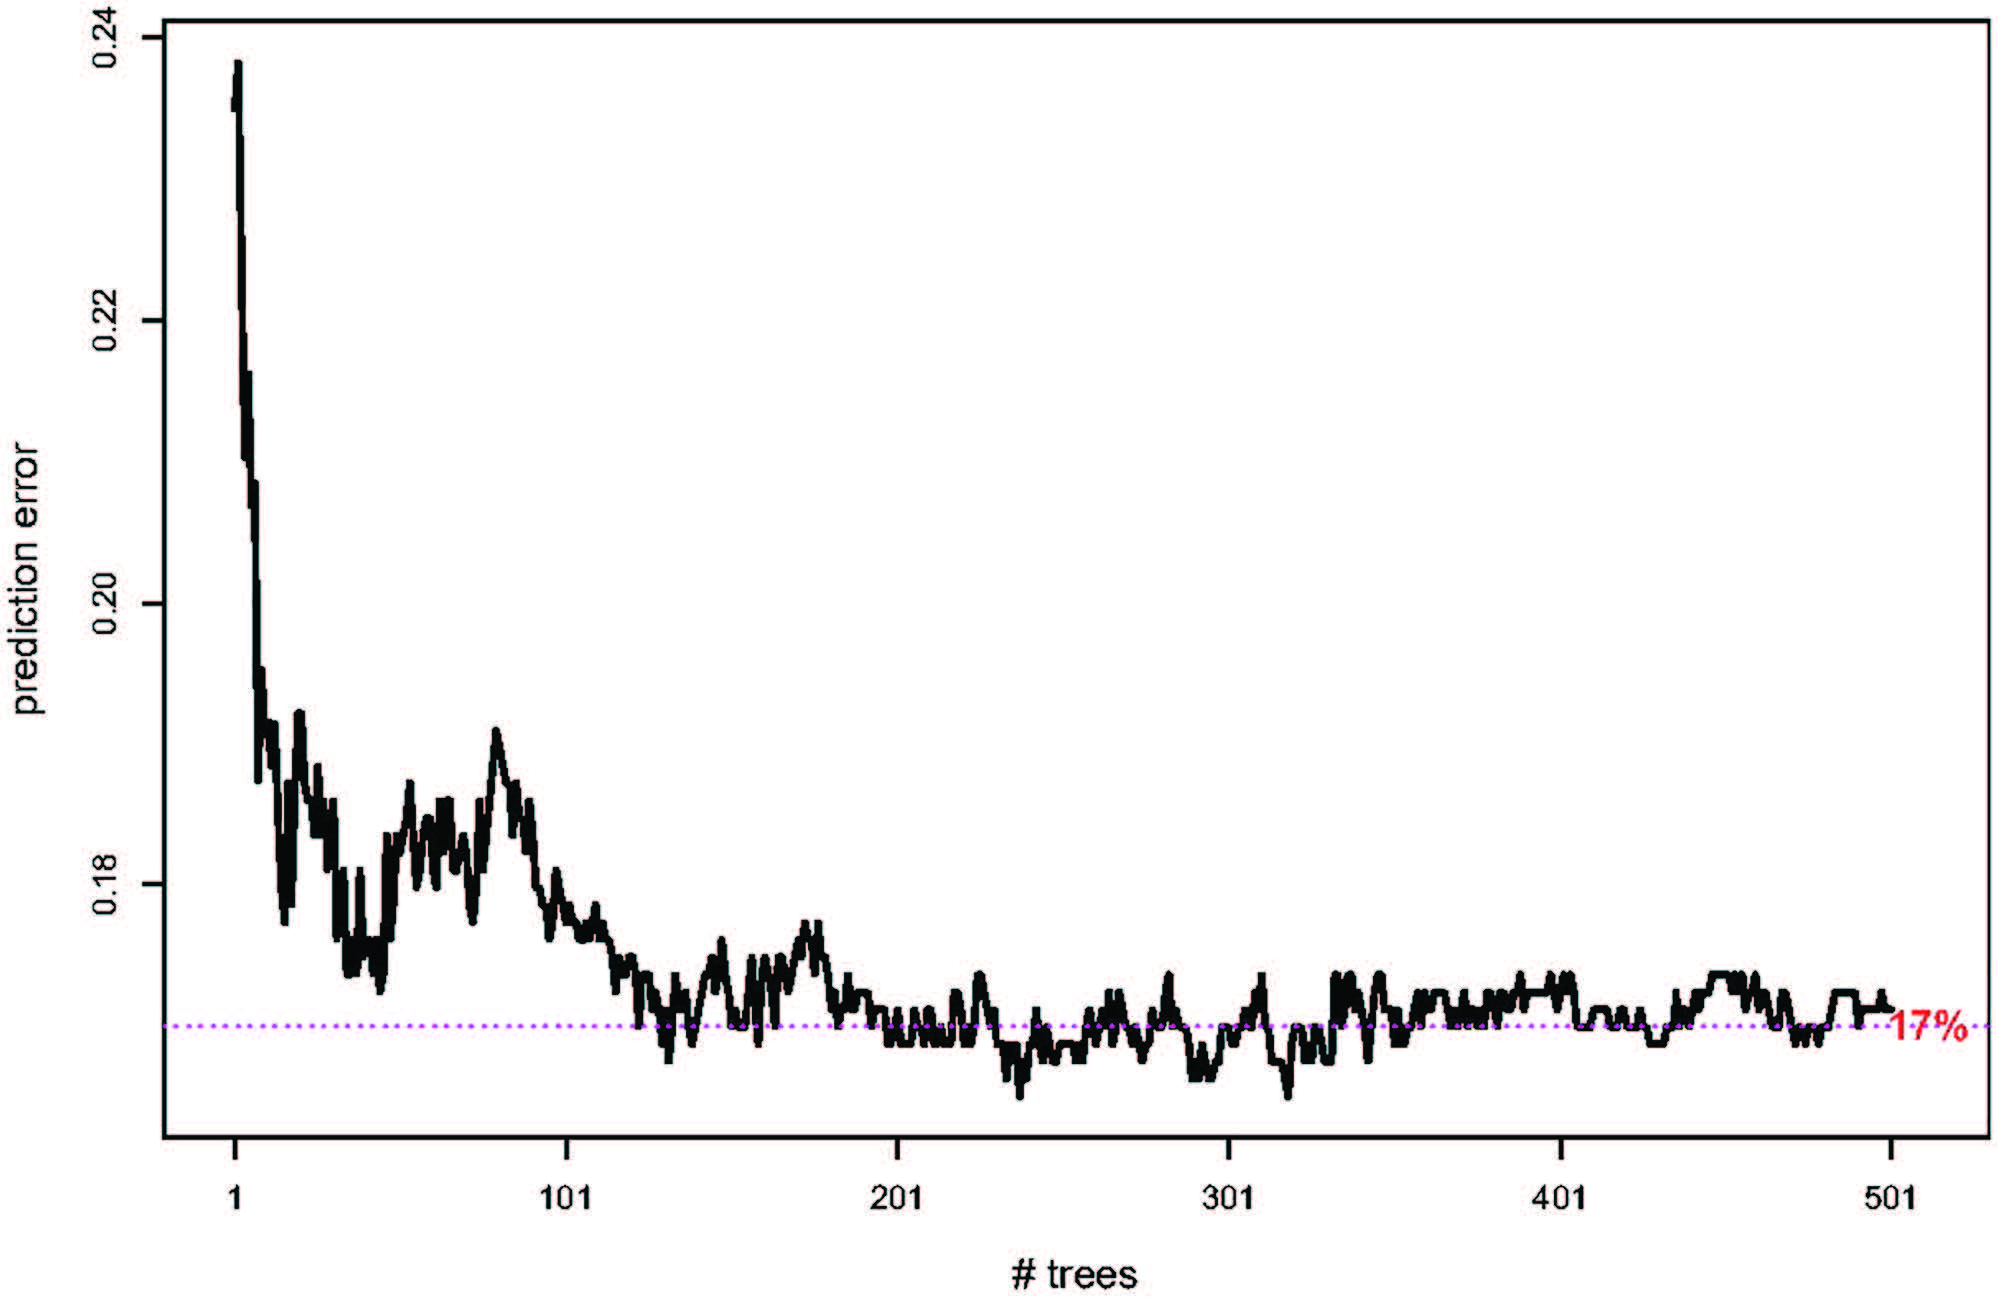
\includegraphics[width=7.7cm]{Fig4.jpg}
		}
		\subfigure[Replot]{
			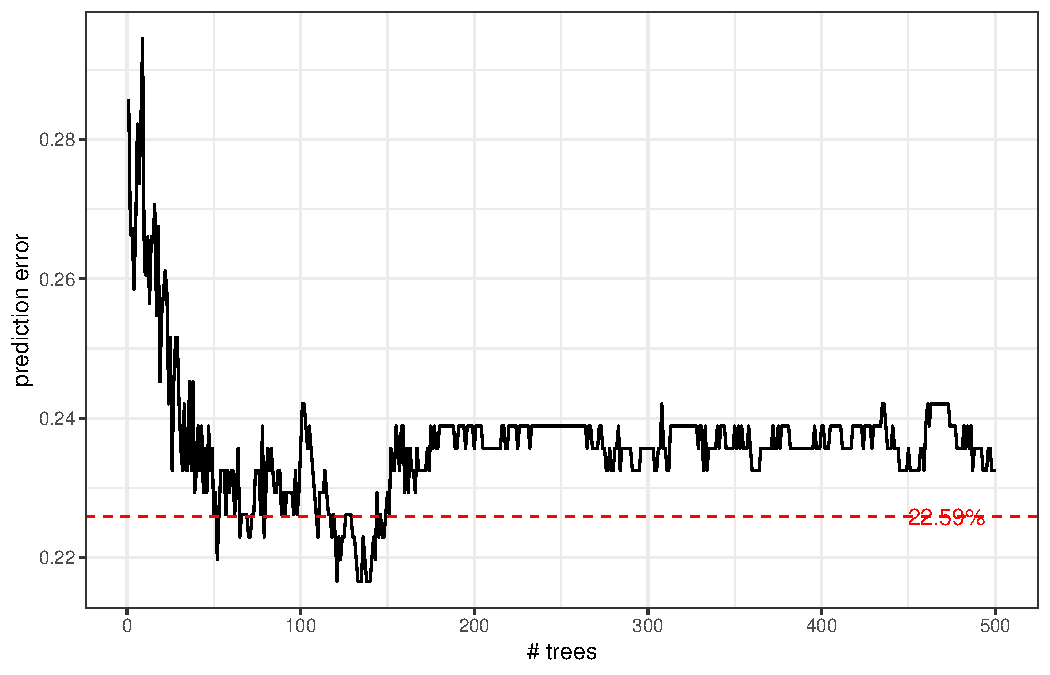
\includegraphics[width=7.7cm]{fig4.pdf}
		}
		\caption{Random forest prediction error rate for neonate data, as a function of number of bootstrapped trees; it has cross-validated error rate 17\%.}
		\label{fig4}
\end{figure}

\section{A Microarray Prediction Problem}

\subsection{Example 5}

纯预测算法有新闻价值的突破涉及到了真正庞大的数据集。在这个例子中并没有提供超大规模的数据,但是作为neonate data的一个小进步,我们将考虑关于前列腺癌症的微阵列研究(microarray study of prostate cancer)。这个研究中有$n=102$个男性,其中52个是癌症患者(cancer patients),50个是正常对照者(normal controls)。用一组$p=6033$的基因来衡量每个男性的基因表达水平:
\begin{align}
x_{i j}=\text { activity of } j \text { th gene for } i \text { th man, }
\end{align}
其中$i=1, 2, \ldots, 102$,$j = 1, 2, \ldots, 6033$。

首先利用random forest对微阵列数据进行预测,normal或cancer。按照标准程序,102名男性被随机分为大小均为51的训练集和测试集,其中有25名正常对照者和26名癌症患者。

图(\ref{fig5})绘制了随着random forest trees数量的增加,在测试集上的预测错误率的结果。100棵树之后,测试集的错误率为2\%。这个表现是十分出色的!这并不是一个特别幸运的结果。随后进行了100次训练集/测试集样本随机分割,每次都重复图(\ref{fig5})中的random forest预测,并计算测试集中预测错误的数量。如表(\ref{table2})所示。
\begin{figure}[H]
		\centering
		\subfigure[Efron's article]{
			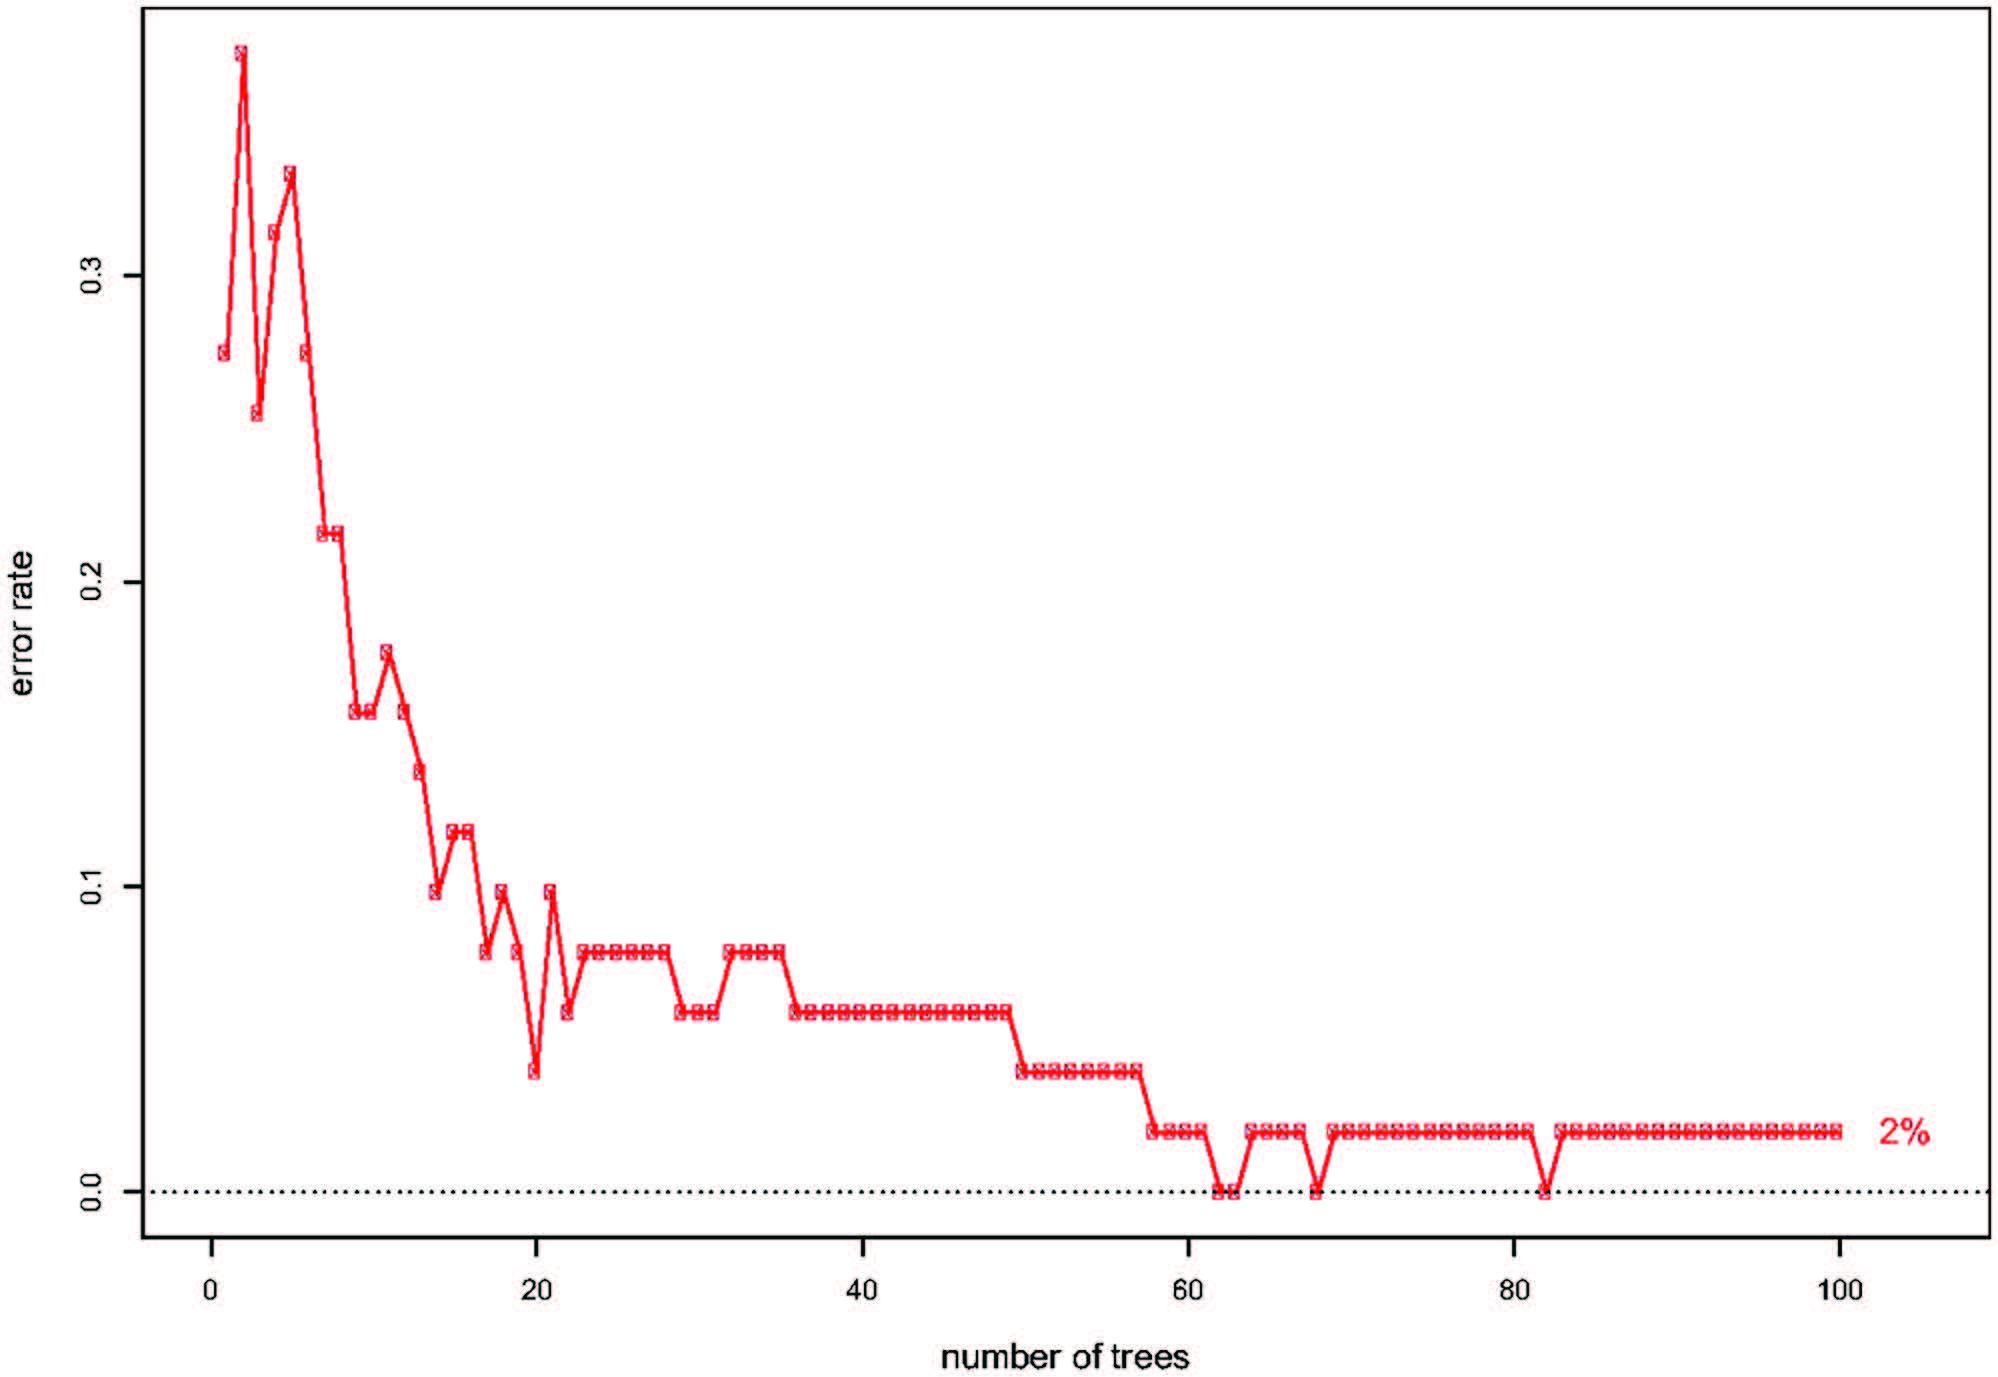
\includegraphics[width=7.7cm]{Fig5.jpg}
		}
		\subfigure[Replot]{
			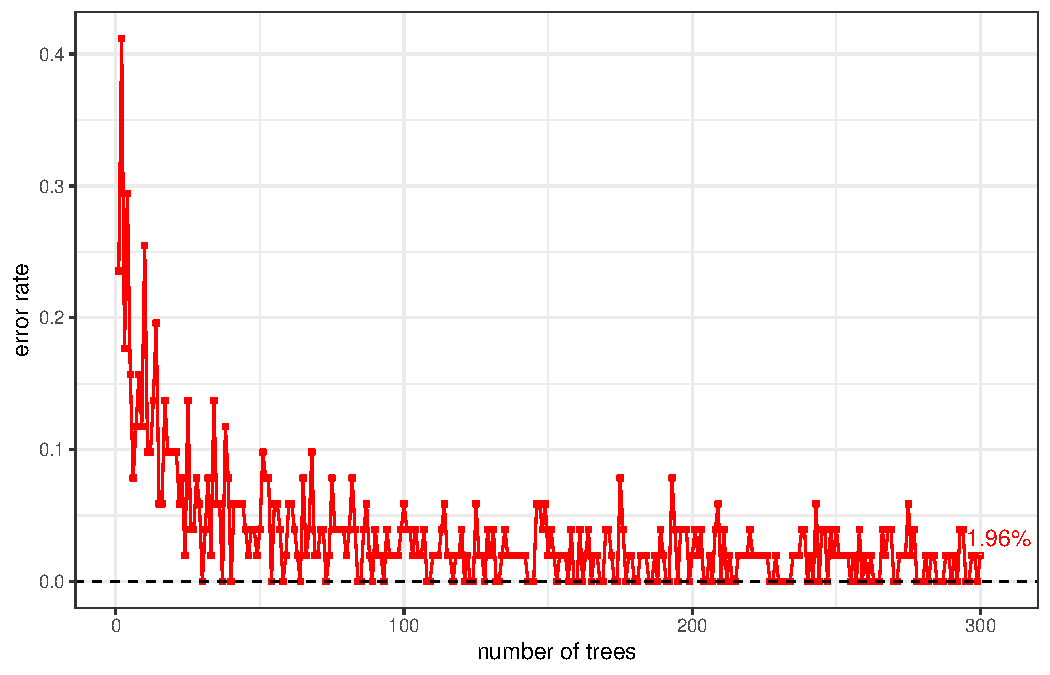
\includegraphics[width=7.7cm]{fig5.pdf}
		}
		\caption{Test set error rate for random forests applied to prostate cancer microarray study, as a function of number of bootstrap trees.}
		\label{fig5}
\end{figure}

\begin{table}[H]
    \centering
    \caption{Number of random forest test set errors in \\100 random training/test splits of prostate data.}
    \label{table2}
    \begin{tabular}{llllllll}
    	\toprule
        Errors & 0 & 1 & 2 & 3 & 4 & 5 & 7 \\
        Frequency & 3 & 26 & 39 & 12 & 5 & 4 & 1 \\
        \midrule
        Re\_Errors & 0 & 1 & 2 & 3 & 4 & 5 & 7 \\
        Re\_Frequency & 26 & 36 & 21 & 9 & 5 & 1 & 1 \\
        \bottomrule
    \end{tabular}
\end{table}

一个分类树可以被认为是一个函数$f(x)$,在它的样本空间$\mathcal{X}$中,对与任意的$x$,$f(x)$取值为0或1。图(\ref{fig3})中的树将11维空间$\mathcal{X}$划分为8个矩形区域,其中3个为$y=0$, 5个为$y=1$。如果在第一次分割后就停止的话可以得到一个更简单的函数,在这种情况下,$\mathcal{X}$被划分为两个区域,cpap $<0.6654$和cpap $\geq 0.6654$。这种简单的树被称为“树桩”(stumps)。

由此引出了另一种突出的纯预测方法,boosting。
\begin{figure}[H]
		\centering
		\subfigure[Efron's article]{
			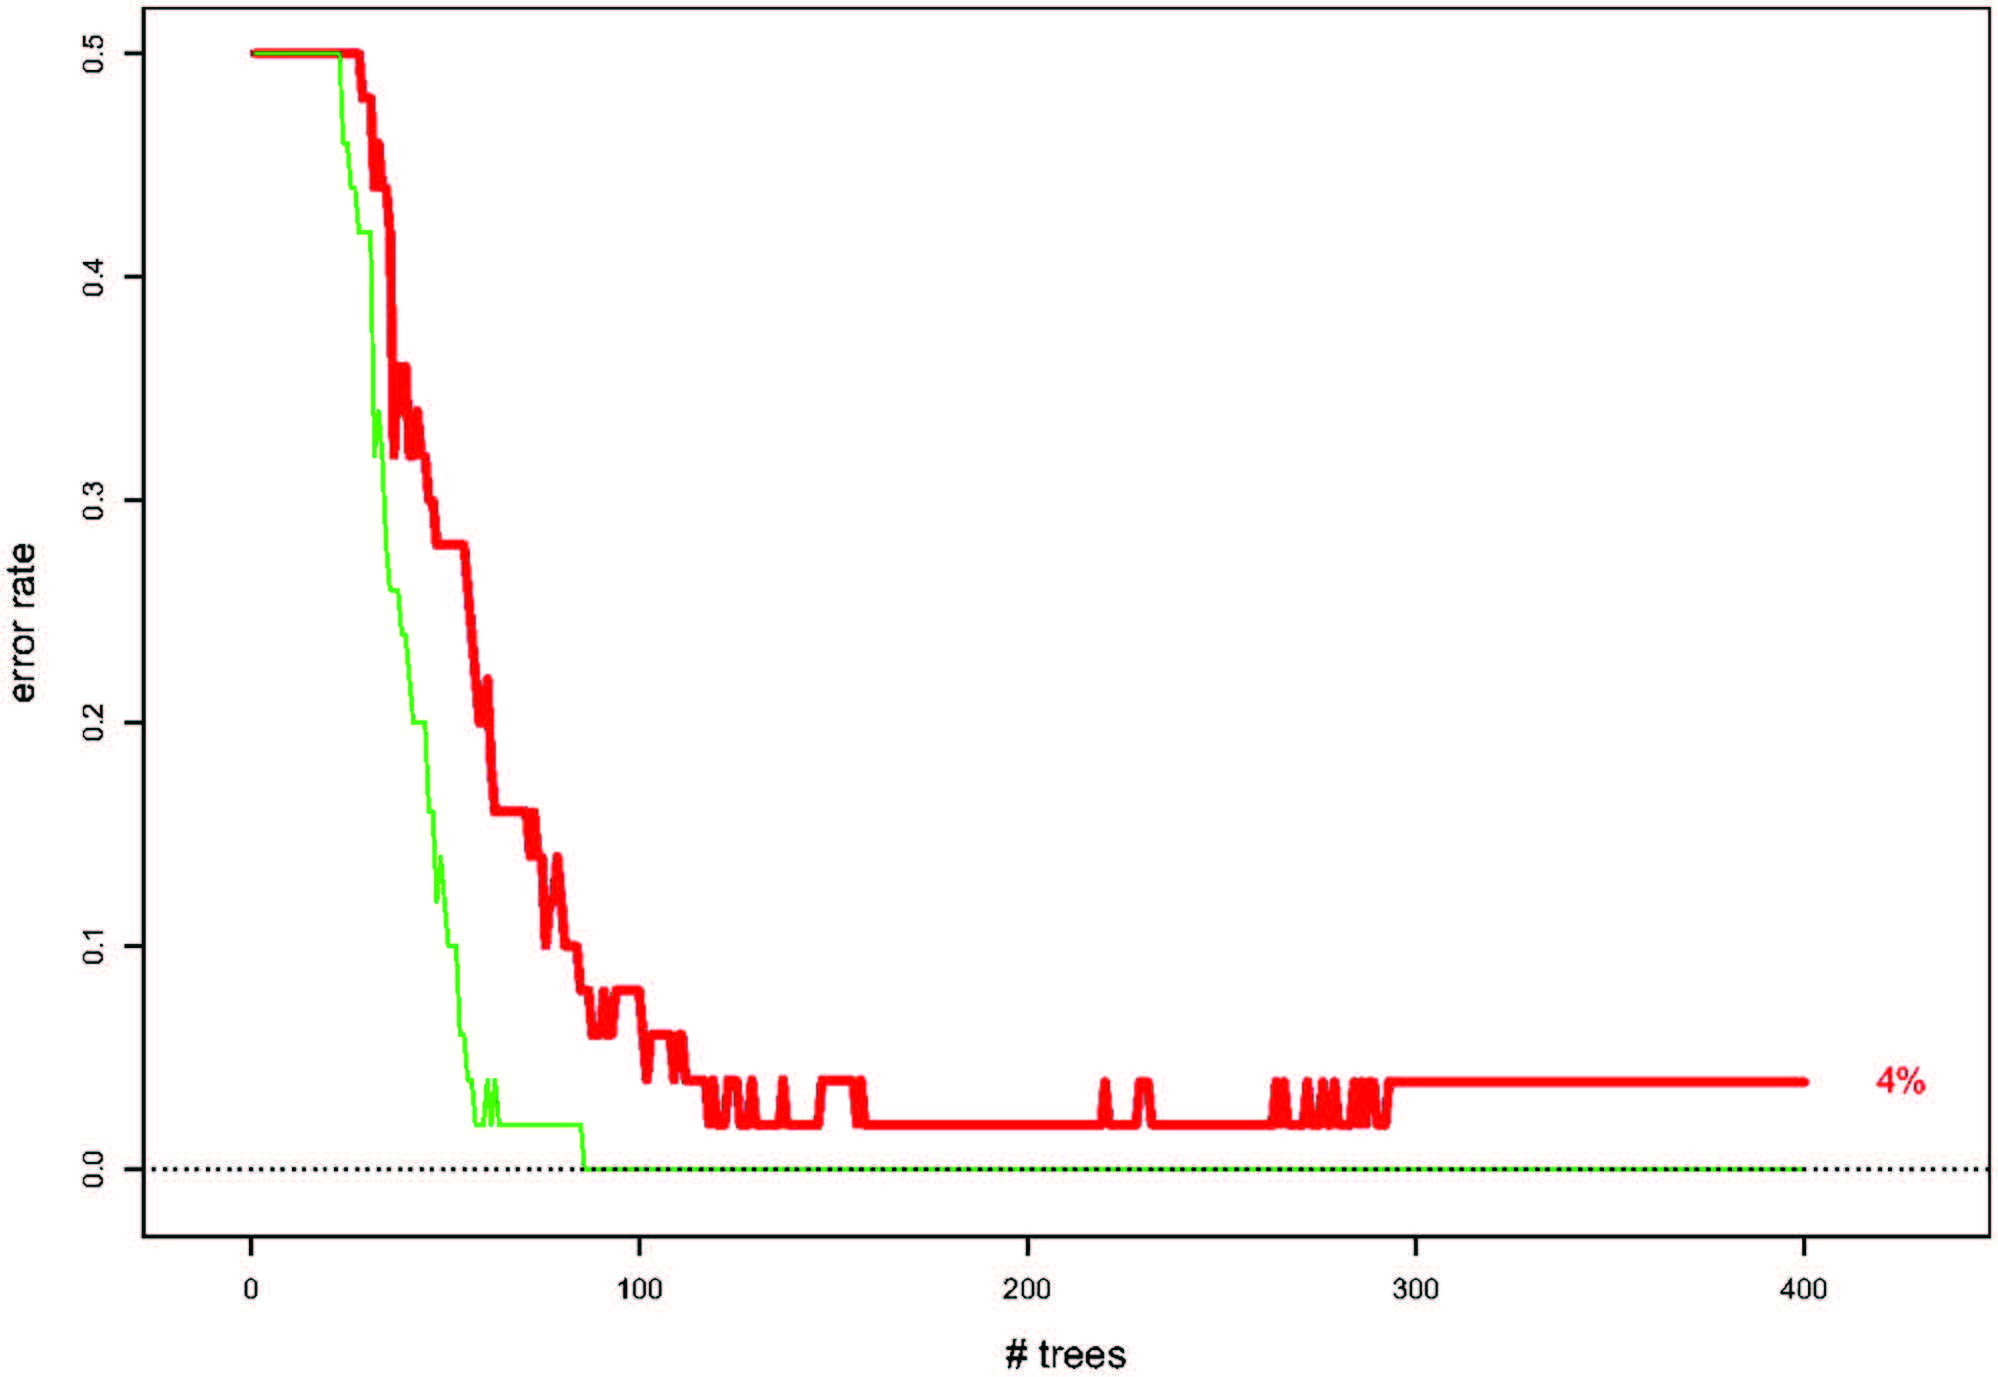
\includegraphics[width=7.7cm]{Fig6.jpg}
		}
		\subfigure[Replot]{
			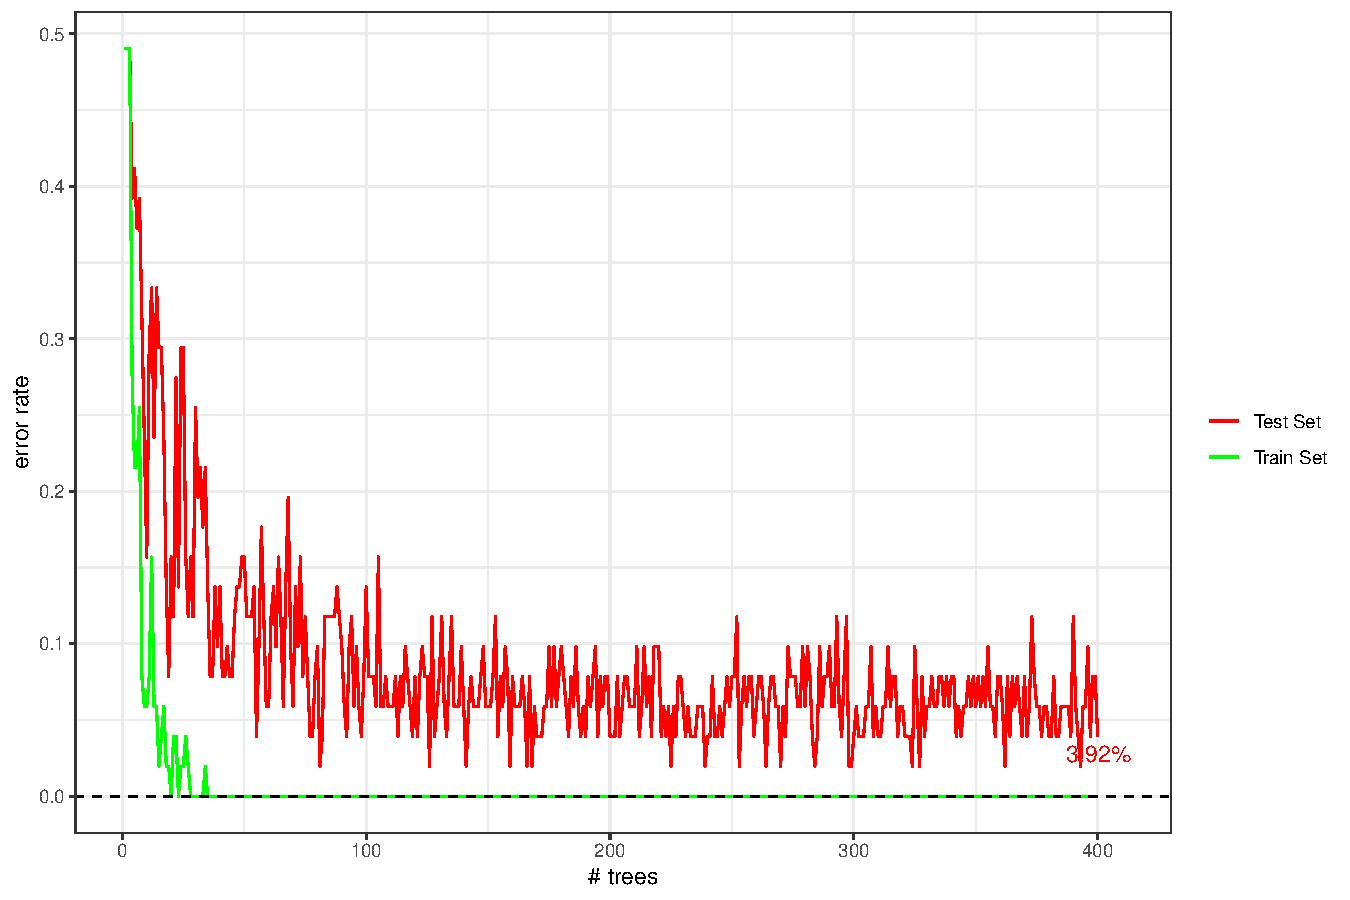
\includegraphics[width=7.7cm]{fig6.pdf}
		}
		\caption{Test set error for boosting algorithm gbm applied to prostate cancer data. Thin curve is training set error, which went to zero at step 86.}
		\label{fig6}
\end{figure}
图(\ref{fig6})展示了gbm (gradient boosting model)算法应用到prostate cancer data中的预测结果。Gbm连续地拟合了分类树的加权和:
\begin{align}
\sum_{k=1}^{K} w_{k} f_{k}(x)
\end{align}
在第$k+1$步,选择树$f_{k+1}(x)$从而最大程度地提升拟合效果,保持较小的权重$w_k$,以避免陷入一个错误的序列。图(\ref{fig6})的结果显示,在400步之后,测试集上的错误率为4\%,这也是一个出色的预测结果。(The examples in \cite{hastie2009elements} show gbm usually doing a little better than random forests.)

In the evocative language of boosting (在boosting的激发性的语言中),进入图(\ref{fig6})结构的stumps被认为是弱学习者(weak learners):他们中的任何一个勉强能将预测错误率降低到50\%以下。无数的弱学习者能够如此有效地结合在一起,这是一个惊喜,也是纯预测算法的核心进步。相比之下,传统的方法侧重于很强的单个预测变量,如表(\ref{table1})中带星号的变量(\textcolor{blue}{In contrast, traditional methods focus on strong individual predictors, as with the asterisks in Table 1})。

在图(\ref{fig6})中比较细的那条曲线表示在训练集上gbm的预测错误率,在第86步时训练集的预测错误率变为0,但此时训练仍在继续,测试集的预测错误率也有所提高。交叉验证计算给出了一些何时停止拟合的提示——这里最好在第200步停止,但这不是一个确定性的问题(Cross-validation calculations give some hint of when to stop the fitting process—here we would have done better to stop at step 200—but it's not a settled question)。

在prostate cancer data上应用神经网络或者深度学习算法的预测效果要比random forest或着gbm差:在测试集上有7个或者8个预测错误,svm算法要更差,在测试集上有11个预测错误。深度学习算法相较其他预测算法是非常错综复杂的,报告显示使用了780,736个参数,这些参数是通过交叉验证设置的内部调节参数(tuning parameters)。这一切的实现要归功于现代强大的计算能力,它是纯预测算法潜在的推动者。

\section{Advantages and Disadvantages of Prediction}

对于我们这些努力在微阵列研究中寻找“重要的”基因的人来说,random forest和gbm几乎完美的prostate cancer预测结果是一个令人不安的惊喜(disconcerting surprise)。不考虑预测算法的惊喜和独创性(ingenuity),一个重要因素可能是prediction比attribution或estimation更容易实现(\textcolor{blue}{Without discounting the surprise, or the ingenuity of the prediction algorithms, a contributing factor might be that prediction is an easier task than either attribution or estimation})。一般情况下,很难去支持这样一个怀疑(suspicion),但有几个例子有助于验证这一点。

对于estimation,假设我们有25个独立同分布的观测,他们来自于期望$\mu$未知的正态分布:
\begin{align}
x_{1}, x_{2}, \ldots, x_{25} \stackrel{\text { ind }}{\sim} \mathcal{N}(\mu, 1)
\end{align}
考虑使用样本均值$\bar{x}$还是样本中位数$\breve{x}$来估计$\mu$。就均方误差而言,样本均值以压倒性的优势胜出,效果超过样本中位数50\%多:
\begin{align}
E\left\{(\breve{x}-\mu)^{2}\right\} / E\left\{(\bar{x}-\mu)^{2}\right\} \doteq 1.57
\end{align}

假设任务换成了对新的数据$X \sim N(\mu, 1)$做预测,样本均值仍然胜出,但是仅仅超过了2\%:
\begin{align}
E\left\{(\breve{x}-X)^{2}\right\} / E\left\{(\bar{x}-X)^{2}\right\} \doteq 1.02
\end{align}

造成这种情况的原因是大部分的预测误差来自于$X$的多变性,这是$\bar{x}$和$\breve{x}$都无法解决的。

Prediction比estimation更容易,至少在更宽容的意义上是这样的。Prediction允许使用效果不好的估计量,如gbm stumps,这对于大规模部署是很方便的。纯预测算法的操作是非参数的,一个附带的好处是不太需要担心估计效率(\textcolor{blue}{The pure prediction algorithms operate nonparametrically, a side benefit of not having to worry much about estimation efficiency})。

为了对比prediction和attribution,我们考虑了微阵列研究的一个理想化版本,有$n$个受试者,其中$n/2$个健康的控制者,$n/2$个为生病的患者:每个受试者提供了$N$个基因的测量值向量,$\bold{X}=\left(X_{1}, X_{2}, \ldots, X_{N}\right)^{t}$,
\begin{align}
\label{Xj}
X_{j} \stackrel{\text { ind }}{\sim} \mathcal{N}\left(\pm \delta_{j} / 2 c, 1\right) \quad(c=\sqrt{n / 4})
\end{align}
$j = 1, 2, \ldots, N$,"plus"表示患者,"minus"表示健康者。$\delta_j$表示基因$j$的效应大小。大多数基因都是$\delta_j = 0$,个数记为$N_0$,但少数的$N_1$个基因的$\delta_j$具有正值$\Delta$:
\begin{align}
N_{0}: \delta_{j}=0 \quad \text { and } \quad N_{1}: \delta_{j}=\Delta
\end{align}

当一个新的人到达,并产生满足条件(\ref{Xj})的微阵列测量值$\bold{X}=\left(X_{1}, X_{2}, \ldots, X_{N}\right)^{t}$,但是没有人知道他是健康的还是患病的。问题来了:在预测变得不可能之前$N_1/N_0$可以多小?答案是当$N_0 \rightarrow \infty$时,如果
\begin{align}
N_{1}=O\left(N_{0}^{1 / 2}\right)
\end{align}
那么准确预测是有可能的。相比之下,实现有效的attribution要求
\begin{align}
N_{1}=O\left(N_{0}\right)
\end{align}

结合弱学习者的prediction策略并不适用于attribution,attribution从定义上看是在寻找较强的单个预测变量。至少在这个例子中,可以公平地说prediction比attribution容易得多。

三种主要的回归类别可以按以下顺序排列:
\begin{align}
\text { prediction } \quad \cdots \quad \text { estimation } \quad \cdots \quad \text { attribution }
\end{align}
estimation处于中心位置,而prediction和attribution彼此之间的距离更远。在传统统计学中,estimation通过$p$值以及置信区间与attribution联系在一起,如表(\ref{table1})所示。从另一个角度来看,当好的估计量可用时,通常也是好的预测量。prediction和estimation都将它们的输出集中在$n\times p$的矩阵$\bold{x}$的$n$侧,而attribution则集中在$p$侧。

\subsection{Example 6}

random forest算法尝试着将prediction和attribution联系在一起,在进行预测的同时,还计算了p个预测变量的重要性得分。图(\ref{fig7})展示了图(\ref{fig5})中prostate cancer预测变量的重要性得分从高到低的排序结果。在$p=6033$个基因中,348个得分为正,这些基因曾被选择作为分割变量。我们是否可以用重要性得分作为attribution,就像表(\ref{table1})中的星号那样(\textcolor{blue}{Can we use the importance scores for attribution, as with the asterisks in Table 1})?

\begin{figure}[H]
		\centering
		\subfigure[Efron's article]{
			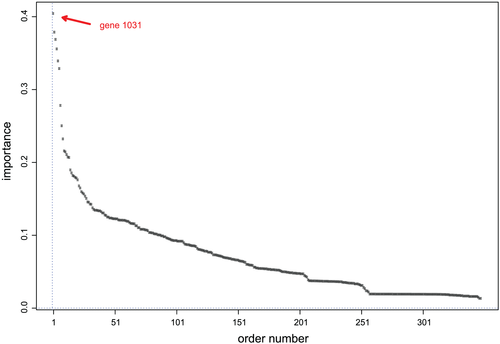
\includegraphics[width=7.7cm]{Fig7.png}
		}
		\subfigure[Replot]{
			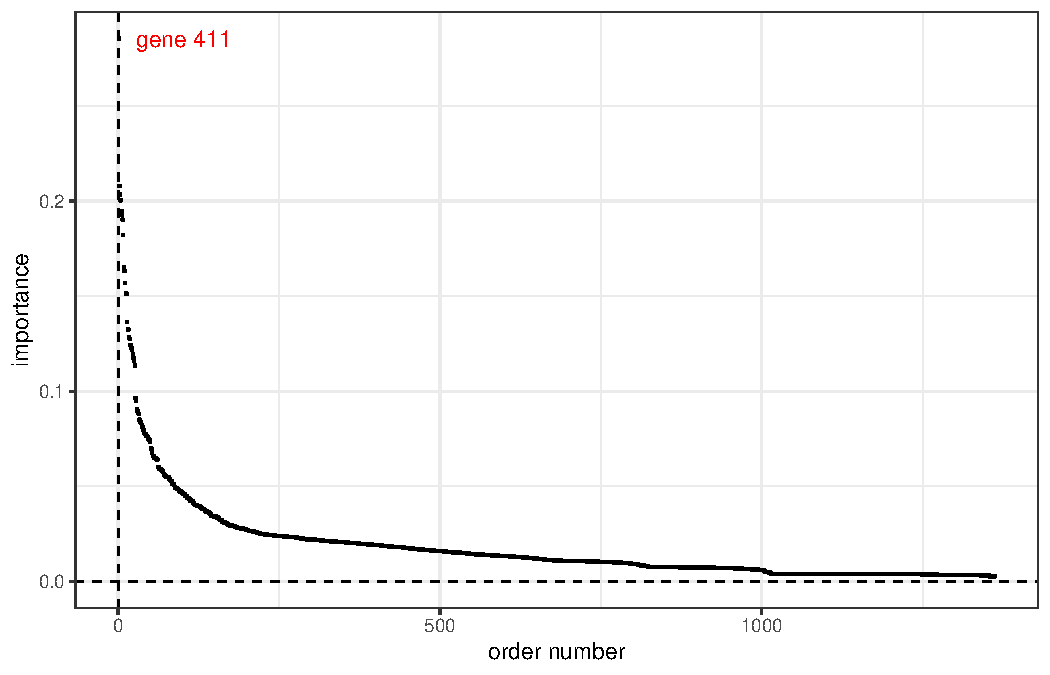
\includegraphics[width=7.7cm]{fig7.pdf}
		}
		\caption{Random forest importance measures for prostate cancer prediction rule of Figure 5, plotted in order of declining importance.}
		\label{fig7}
\end{figure}

在这种情况下,答案似乎是否定的。我从数据集中依次删除重要性得分较高的基因,重新应用random forest算法,如表(\ref{table3})所示,无论去掉多少个重要性得分为正的基因,对于测试集上的预测错误率是相似的。random forest算法基于减少后的数据集仍能给出出色的预测结果。

\begin{table}[H]
    \centering
    \caption{Number of test set errors for prostate cancer random forest predictions, removing top predictors shown in Figure 7.}
    \label{table3}
    \begin{tabular}{lccccccccccccc}
    	\toprule
        \# removed & 0 & 1 & 5 & 10 & 20 & 40 & 80 & 160 & 348 &&&&\\
        \# errors & 1 & 0 & 3 & 1 & 1 & 2 & 2 & 2 & 0 &&&&\\ 
        \midrule
        \# Re\_removed & 0 & 1 & 5 & 10 & 20 & 40 & 80 & 160 & 300 & 500 & 1000 & 3000 & 5000 \\
        \# Re\_errors & 0 & 2 & 0 & 0 & 0 & 1 & 0 & 1 & 2 & 0 & 1 & 2 & 5 \\
        \bottomrule
    \end{tabular}
\end{table}

在这个例子中,弱学习者的预测模型似乎是占优势的。很明显有许多基因与prostate cancer的相关性很弱,但是预测算法可以用这些弱学习者的不同组合来给出近乎完美的预测(\textcolor{blue}{Evidently there are a great many genes weakly correlated with prostate cancer, which can be combined in different combinations to give near-perfect predictions})。如果预测是唯一的目标,这确实是一个优势,但从attribution的角度来看,这是一个劣势。如表(\ref{table1})所示,传统的attribution是在努力识别一小部分有因果关系的协变量(即使不能推断出严格的因果关系)。

\section{The Training/Test Set Paradigm}

\subsection{Example 7}

现代预测方法的一个重要组成部分就是training/test set paradigm:数据集$\bold{d}$被分割为训练集$\bold{d}_{\text{train}}$和测试集$\bold{d}_{\text{test}}$,使用训练集$\bold{d}_{\text{train}}$计算得到一个预测准则$f(x, \bold{d}_{\text{train}})$,最后使用$f(x, \bold{d}_{\text{train}})$对测试集$\bold{d}_{\text{test}}$进行预测,得到预测错误率的可靠估计,但可靠并不意味着完美。

在第4节中对prostate cancer microarray就采用了这种paradigm,应用random forest算法得到了一个非常小的预测错误率2\%,这样的预测结果对于我来说是非同寻常的,那么为什么不利用这一预测准则,基于一组新的6033个基因表达测量结果去诊断某人是否患有prostate cancer?下面的例子说明了这可能会出错。

在第4节中,prostate cancer data训练集和测试集的获取是通过将102名男性随机地分为两个51人的小组,每组25名正常对照者和26名癌症患者。文献中强调随机化(randomization)是为了防止产生偏差。在这个例子中我违背了randomization,重复prostate cancer microarray的研究,这次选择了ID号最低的25名正常对照者和26名癌症患者作为训练集。测试集则是剩下的51名ID较高的受试者,同样包括25名正常对照者和26名癌症患者。

在重新对prostate cancer microarray的分析中,random forest的表现不如图(\ref{fig5})所示:这次在测试集上的错误率高达24\%,而不是之前的2\%,如图(\ref{fig8})所示。gbm的表现也是一样的糟糕,产生的预测错误率为28\%,如图(\ref{fig9})所示。
\begin{figure}[H]
		\centering
		\subfigure[Efron's article]{
			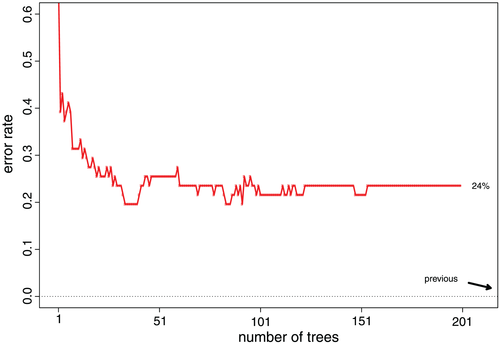
\includegraphics[width=7.7cm]{Fig8.png}
		}
		\subfigure[Replot]{
			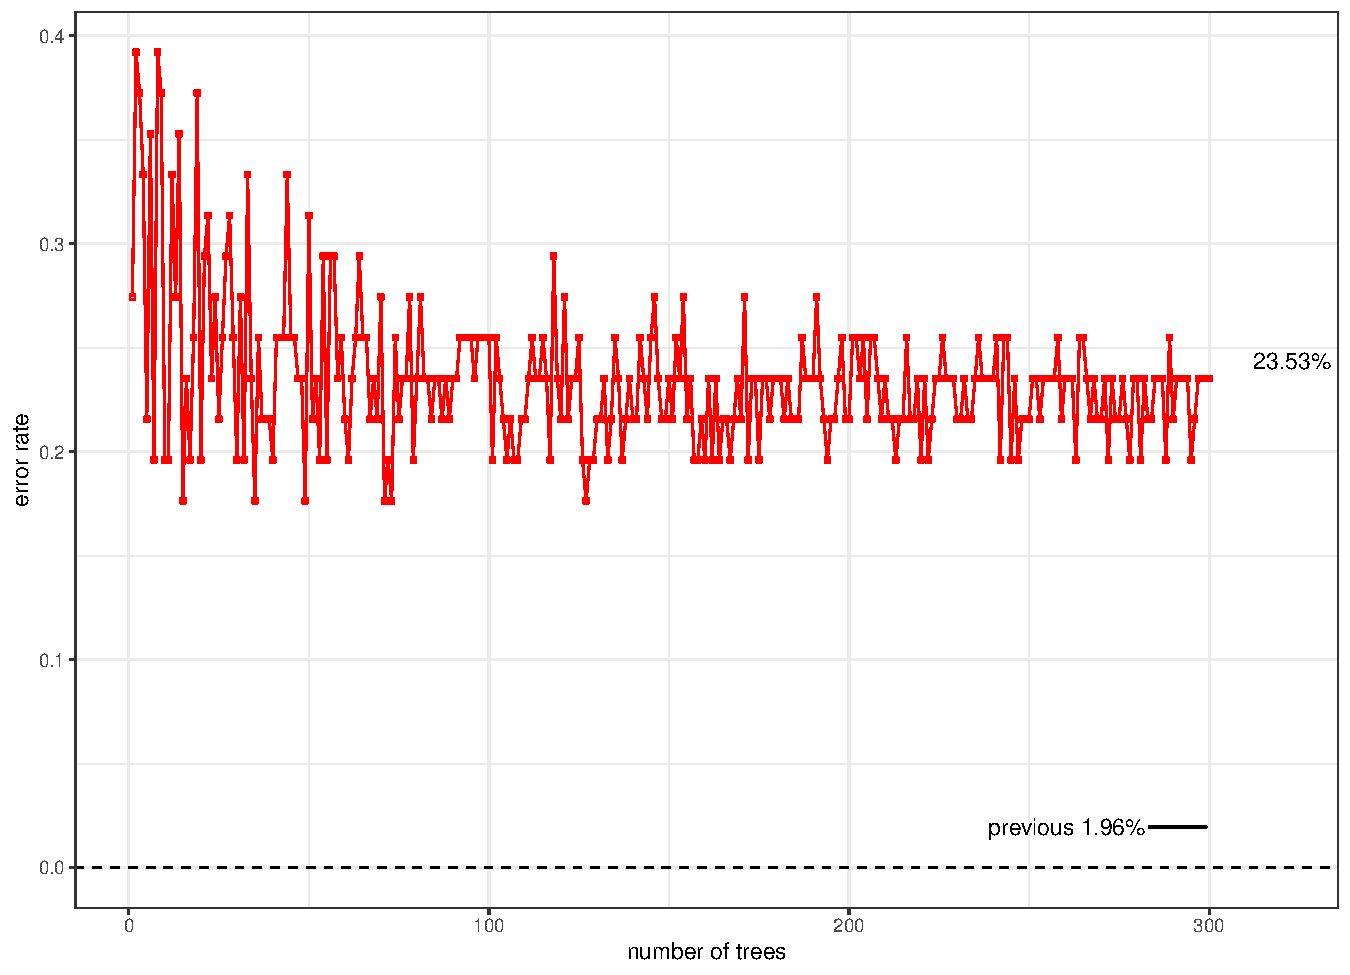
\includegraphics[width=7.7cm]{fig8.pdf}
		}
		\caption{randomForest test set error for prostate cancer microarray study, now with training/test sets determined by early/late ID number. Results are much worse than in Figure 5.}
		\label{fig8}
\end{figure}

\begin{figure}[H]
		\centering
		\subfigure[Efron's article]{
			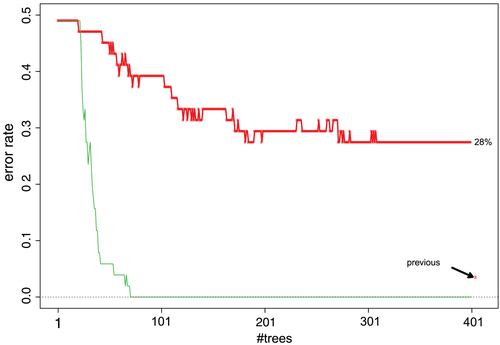
\includegraphics[width=7.7cm]{Fig9.png}
		}
		\subfigure[Replot]{
			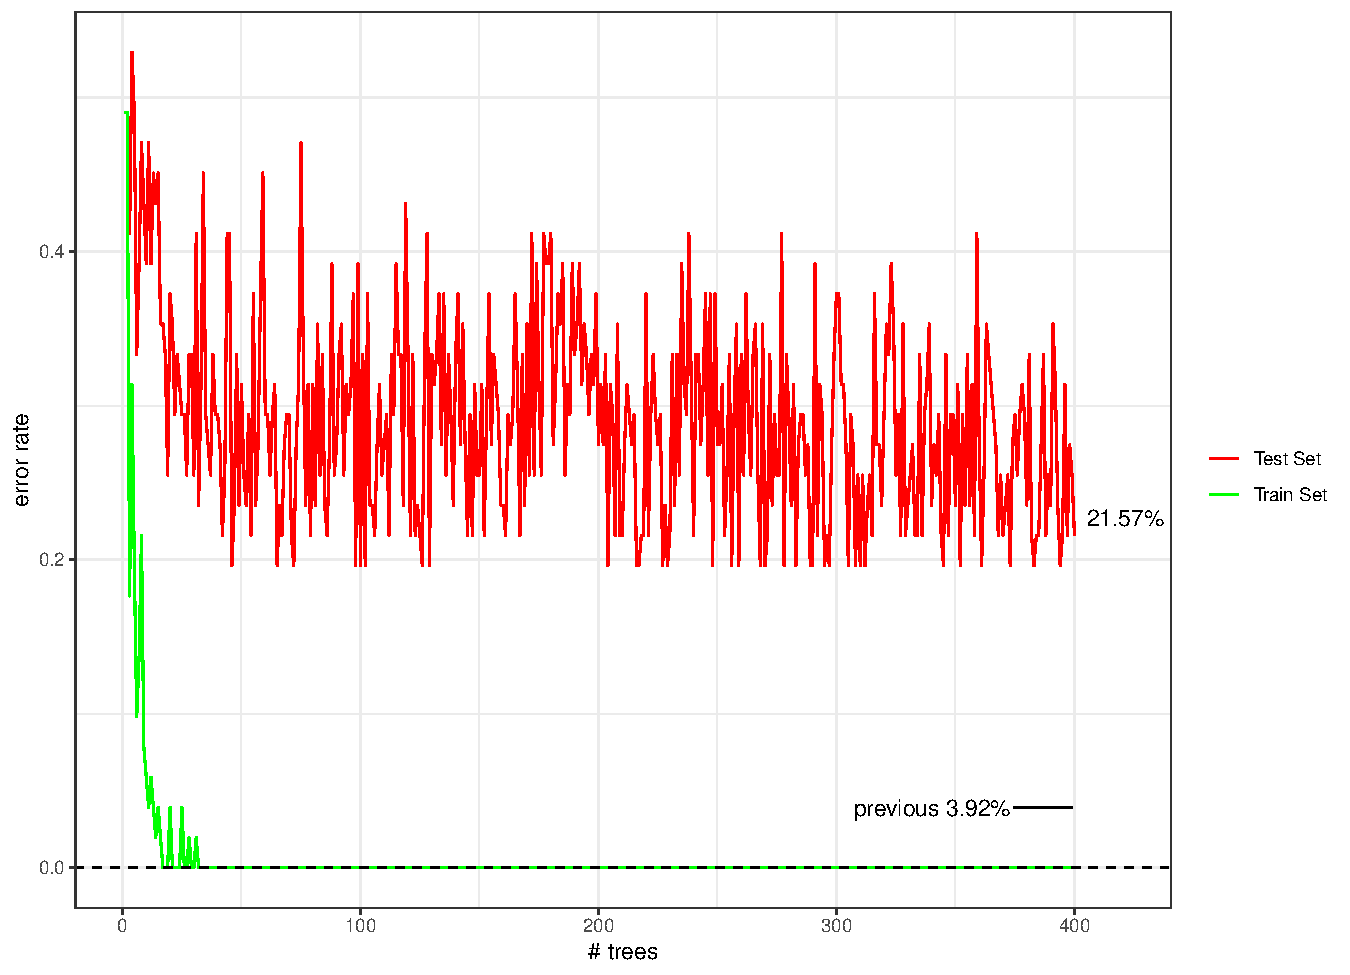
\includegraphics[width=7.7cm]{fig9.pdf}
		}
		\caption{gbm test set error, early/late division; compare with Figure 6. Going on to 800 trees decreased error estimate to 26\%. Training set error rate, thin curve, was zero after step 70 but test error rate continued to decline. See the brief discussion in Criterion 5 of Section 8.}
		\label{fig9}
\end{figure}

为什么现在的预测效果这么差?从检查中来看并不是很明显,但prostate研究对象可能是按照所列的顺序收集的,并且随着时间的推移会有一些小的方法上的差异。也许所有进入random forest和gbm的弱学习者都非常容易受到这种差异的影响。有关prediction的相关文献用概念"drift"作为这类麻烦的标签,一个臭名昭著的例子是Google flu predictor,它打败了CDC (疾控中心)数年,然后惨败。通过随机选择来选取测试集听起来很谨慎,但它肯定会隐藏一些drift effects。

"drift"这一概念让我们陷入这样一个问题:我们的各种回归方法,无论是新的还是旧的,应该告诉我们什么?从历史上看,科学一直在寻找支配我们宇宙的潜在真理,就像牛顿定律。在物理学和天文学中,永恒的部分是十分清楚的,$E=mc^2$,Hubble's law,或许在医学和生物学中也是如此,例如DNA和血液循环。但是,现代科学已经进入了真理可能更具偶然性的领域,如经济学、社会学和生态学。

传统的estimation和attribution旨在获得超越即时(immediate)数据集的长期结果(\textcolor{blue}{traditional estimation and attribution usually aim for long-lasting results that transcend the immediate datasets})。在第2节的surface plus noise模型中,surface扮演着真理的角色——至少永恒到足以证明在为最接近的估计而努力着(at least eternal enough to justify striving for its closest possible estimation)。

在表(\ref{table1})的neonate例子中,我们希望像gest和ap这样的星标预测变量在未来的研究中继续发挥重要作用。在第2年的数据中,只有$n=246$个新生儿。对第2年的数据进行了同样的逻辑回归模型,得出的系数估计值与第1年的值相当相似,见表(\ref{table4})。

\begin{table}[H]
    \centering
    \caption{Comparing logistic regression coefficients for neonate data for year 1 (as in Table \ref{table1}) and year 2; correlation coefficient 0.79}
    \label{table4}
    \begin{tabular}{llllllllllll}
    \toprule
    & gest & ap & bwei & resp & cpap & ment & rate & hr & head & gen & temp \\
    \midrule 
    Year 1 & –0.47 & –0.58 & –0.49 & 0.78 & 0.27 & 1.10 & –0.09 & 0.01 & 0.1 & 0.00 & 0.02 \\ 
    Year 2 & –0.65 & –0.27 & –0.19 & 1.13 & 0.15 & 0.41 & –0.47 & –0.02 & –0.2 & –0.04 & 0.16 \\ 
    \bottomrule
    \end{tabular}
\end{table}

没有什么能排除纯预测算法寻求永恒真理的可能性,但它们最著名的还是应用在更短暂的现象中:信用评分、Netflix电影推荐、面部识别、Jeopardy! competitions。预测算法的一大优势是能够从大量混杂的数据集中提取信息,即使只是为了短期使用。对测试集进行随机选取在这种背景下是有意义的,只要估计的错误率在当前数据集的有限范围之内,或者不会在有限范围之外太远。

\subsection{Example 8}

接下来是一个人为设计的微阵列的例子,所有的预测变量都是短暂的:$n=400$名受试者参与研究,每天在Treatment和Control之间交替到达一个,每个受试者测量一个$p=200$的基因微阵列。$400 \times 200$数据矩阵$\bold{x}$的每条数据是相互独立的:
\begin{align}
\begin{array}{c}
x_{i j} \stackrel{\text { ind }}{\sim} \mathcal{N}\left(\mu_{i j}, 1\right) \text { for } i=1,2, \ldots, 400 \text { and } \\
j=1,2, \ldots, 200
\end{array}
\end{align}

大多数的$\mu_{ij}=0$,但是偶尔会有一个基因有30天的活跃片段(active episode),在这期间:
\begin{equation}
\label{choose1}
\mu_{i j}=2 \quad \text { for Treatment } \quad \text { and } \quad-2 \quad \text { for Control }
\end{equation}
或
\begin{equation}
\label{choose2}
\mu_{i j}=2 \quad \text { for Control } \quad \text { and } \quad-2 \quad \text { for Treatment }
\end{equation}
在(\ref{choose1})和(\ref{choose2})之间的选择是随机的,每一个活跃片段的开始日期也是随机的。每个基因的平均活跃次数为1次,如图(\ref{fig10})所示,黑色的线段表示所有的活跃时期。
\begin{figure}[H]
		\centering
		\subfigure[Efron's article]{
			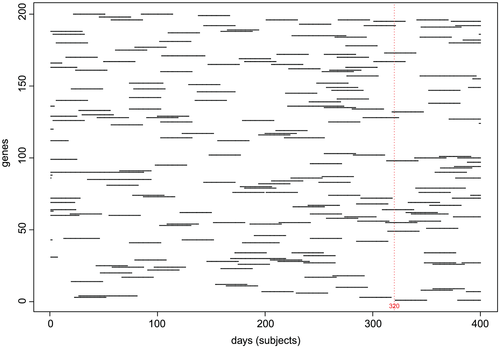
\includegraphics[width=7.7cm]{Fig10.png}
		}
		\subfigure[Replot]{
			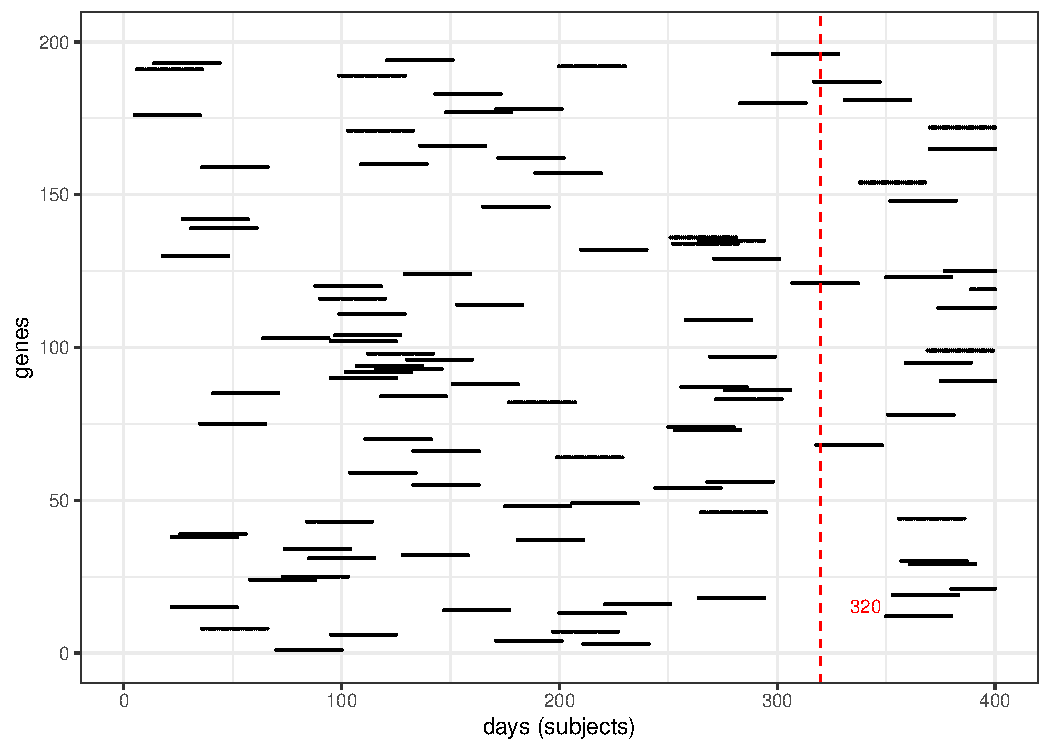
\includegraphics[width=7.7cm]{fig10.pdf}
		}
		\caption{Black line segments indicate active episodes in the hypothetical microarray study. (Matrix transposed for typographical convenience.)}
		\label{fig10}
\end{figure}

接下来对这组人为构造的数据进行random forest预测,训练集和测试集的分割方法分别采用随机分割法和先后次序分割法。结果展示在图(\ref{fig11})的左右两边,左图显示随机分割所得的测试集预测错误率为19\%,右图显示先后次序分割法所得的测试集预测错误率为45\%。

在这种情况下,很容易看出问题出在哪里。从任何一天的测量结果中,都有可能从附近几天的active episode responses来预测Control或Treatment。这适用于随机分割法,其中大部分的测试日期将与训练日期混杂在一起。但对于先后次序分割法(early/late division)就不是这样了,因为大部分的测试日期都与训练集日期相差甚远。换句话说,插值(interpolation)预测比外推(extrapolation)预测更容易。

\begin{figure}[H]
		\centering
		\subfigure[Efron's article]{
			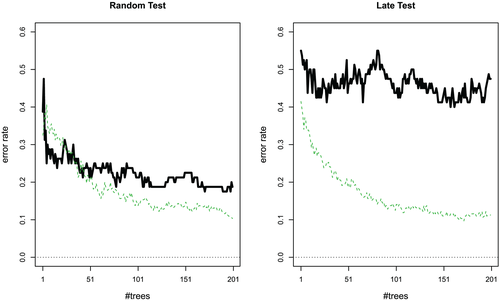
\includegraphics[width=15cm]{Fig11.png}
		}\\
		\subfigure[Replot]{
			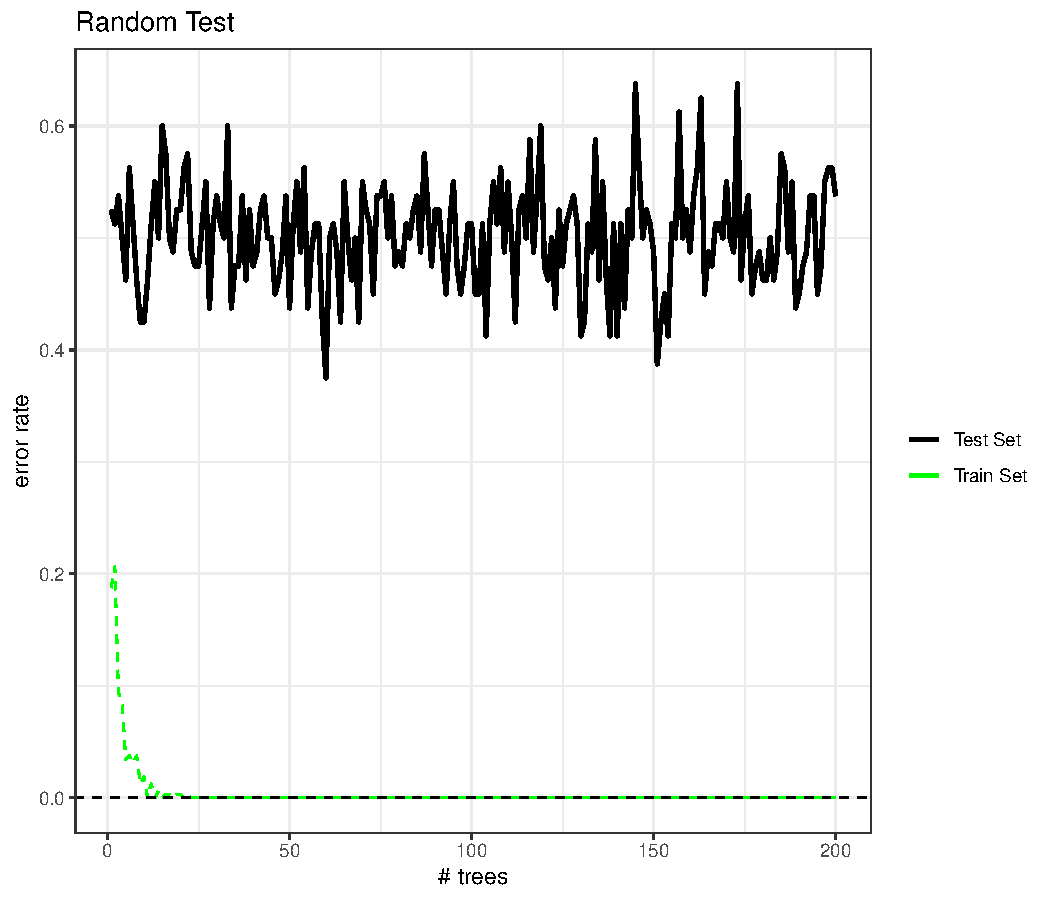
\includegraphics[width=7.7cm]{fig111.pdf}
		}
		\subfigure[Replot]{
			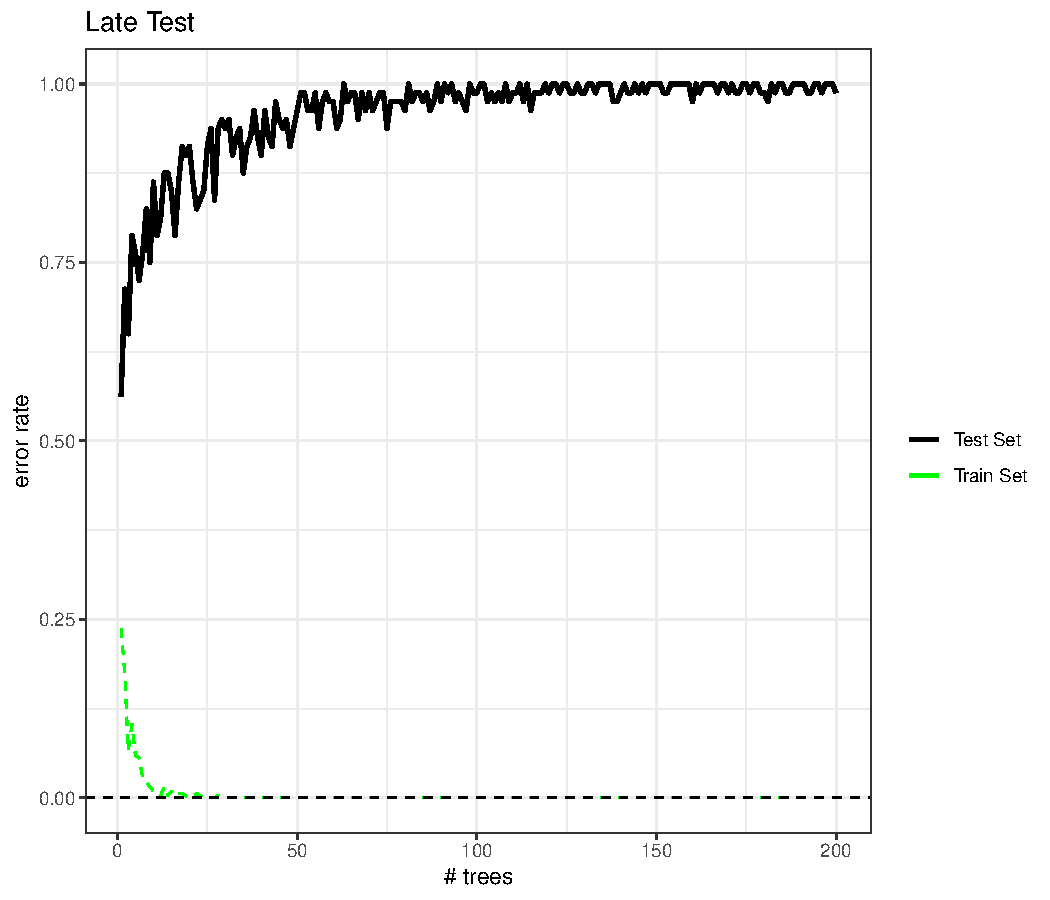
\includegraphics[width=7.7cm]{fig112.pdf}
		}
		\caption{randomForest prediction applied to contrived microarray study pictured in Figure 10. Left panel: Test set of size 80, selected randomly from 400 days; heavy black curve shows final estimated test error rate of 19\%. Right panel: Test set days 321–400; now error rate estimate is 45\%. Light dotted curves in both panels are training set errors.)}
		\label{fig11}
\end{figure}

通常我们可以从训练集或测试集误差估计中学到什么?回到公式(\ref{data}),通常的假设是数据对$(x_i, y_i)$是独立同分布的,来自于某个在$p$维空间上的概率分布$F$:
\begin{align}
\left(x_{i}, y_{i}\right) \stackrel{\text { iid }}{\sim} F \quad \text { for } \quad i=1,2, \ldots, n
\end{align}

大小为$n_0$的训练集$\bold{d}_0$和大小为$n_1 = n-n_0$的测试集$\bold{d}_1$被选择,得到预测准则$f(x, \bold{d}_0)$并应用到$\bold{d}_1$上,从而得到了一个误差估计:
\begin{align}
\label{model F}
\widehat{\text{Err}}_{n_{0}}=\frac{1}{n_{1}} \sum_{d_{1}} L\left(y_{i}, f\left(x_{i}, \mathbf{d}_{0}\right)\right)
\end{align}
$L$是某种误差函数,如均方误差或计数误差。然后基于模型(\ref{model F}),$\widehat{\text{Err}}_{n_{0}}$的无偏估计为:
\begin{align}
\operatorname{Err}_{n_{0}}(F)=E_{F}\left\{\widehat{\text{Err}}_{n_{0}}\right\}
\end{align}

"drift"这一概念可以被解释为数据生成机制(\ref{model F})的变化,比如分布$F$变化为一些新的分布$\tilde{F}$,这可能是图(\ref{fig8})和(\ref{fig9})中prostate cancer预测效果很差的罪魁祸首,传统的预测方法也容易受到这种变化的影响。在neonate data研究中,基于第1年数据的逻辑回归预测模型所得的交叉验证错误率为20\%,而应用于第2年数据时,交叉验证错误率增加到了22\%。

对于图(\ref{fig10})和图(\ref{fig11})人为构造的例子来说,情况更加复杂,其中模型(\ref{model F})并不严格适用。其中有效的预测变量是短暂的,只在短时间内活跃。一个合理的推测(但仅此而已)是,纯预测算法的弱学习者倾向于短暂性,或者至少比传统方法中青睐的主要预测变量更倾向于短暂性(\textcolor{blue}{A reasonable conjecture (but no more than that) would say the weak learners of the pure prediction algorithms are prone to ephemerality, or at least are more prone than the "main effects" kind of predictors favored in traditional methodology})。不管这是不是真的,我觉得通过随机选择来构建训练集和测试集是有一些危险的,必须对他们的误差估计持保留态度。从实际操作上来讲,我很惶恐向一个关心prostate cancer的朋友推荐图(\ref{fig5})中的random forest预测准则。

这不仅仅是一种假想出来的担忧。在2019年的文章"Deep Neural Networks are
Superior to Dermatologists in Melanoma Image Classification"中(深度神经网络在黑色素瘤图像分类方面优于皮肤科医生),\cite{brinker2019deep}证明了标题中所说的。作者非常谨慎,建议在未来进行研究加以验证。此外,他们承认了随机选取测试集的局限性,以及算法中某些预测变量可能是短暂的。对于任何这种诊断算法的严格使用,频繁的更新都是十分必要的。

\section{Smoothness}

\subsection{Example 9}

牛顿的微积分与牛顿的运动定律并不是一个令人愉悦的巧合。如拉普拉斯所描述的那样,牛顿的世界是一个无限平滑的世界,在这个世界里,微小的因果变化会产生微小的结果变化,并且许多阶导数都有物理意义。传统统计方法的参数化模型执行了smooth-world paradigm。回头看第2节的图(\ref{fig1}),我们可能不同意cholostyramine三次回归曲线的确切形状,但响应结果的平滑性似乎是无可争辩的。

响应结果的平滑性没有包含在纯预测算法中,左图(\ref{fig12})展示了random forest的估计结果。它大致遵循OLS三次曲线,但呈现锯齿状并且绝对是不平滑的。在右边的图中,gbm算法给出了一条锯齿较少的曲线,但仍然有大量的局部不连续。

\begin{figure}[H]
		\centering
		\subfigure[Efron's article]{
			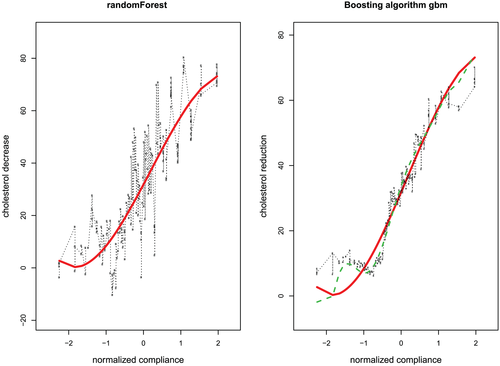
\includegraphics[width=15cm]{Fig12.png}
		}\\
		\subfigure[Replot]{
			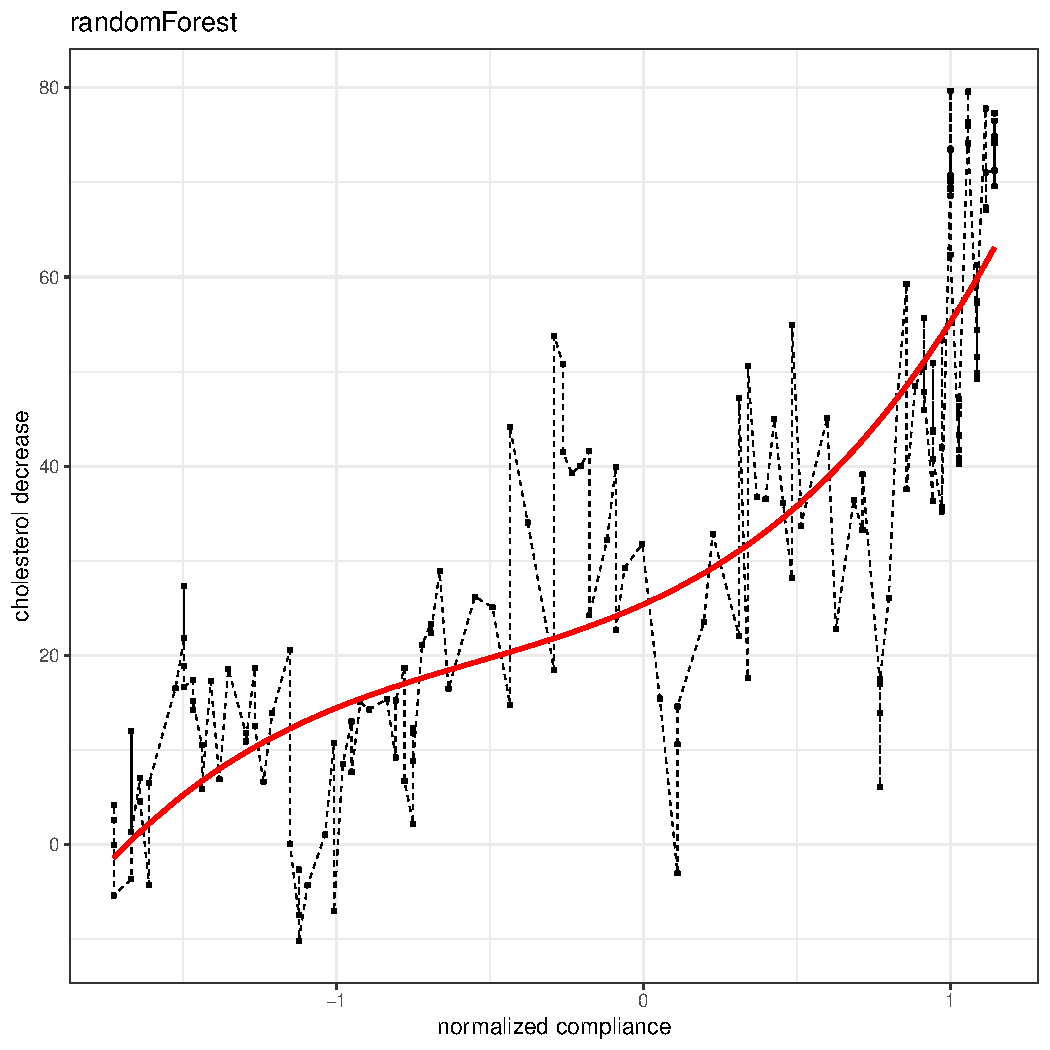
\includegraphics[width=7.7cm]{fig121.pdf}
		}
		\subfigure[Replot]{
			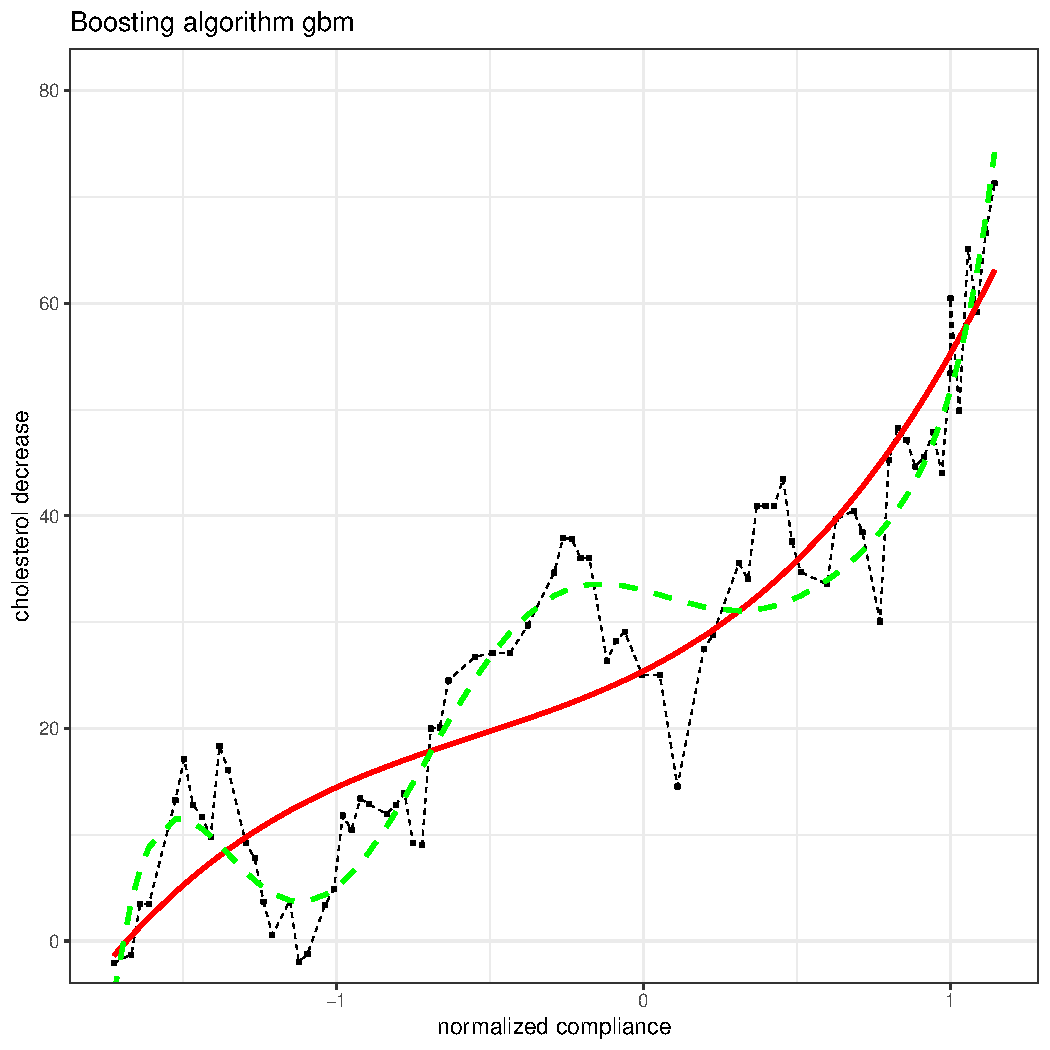
\includegraphics[width=7.7cm]{fig122.pdf}
		}
		\caption{randomForest and gbm fits to the cholostyramine data of Figure 1 in Section 2. Heavy curve is cubic OLS; dashed curve in right panel is 8th degree OLS fit.)}
		\label{fig12}
\end{figure}

\subsection{Example 10}

接下来考虑supernova data:记录了$n=75$个supernovas的绝对亮度$y_i$,以及在$p=25$个不同波长下的光谱能量测量值$x_i$,因此数据集是:
\begin{align}
\label{supernova data}
	\bold{d} = \{\bold{x}, \bold{y} \}
\end{align}
其中$\bold{x}$为$75 \times 25	$,$\bold{y}$是一个75维向量。经过一些预处理,一个合理的模型是:
\begin{align}
y_{i} \stackrel{\text { ind }}{\sim} \mathcal{N}\left(\mu_{i}, 1\right)
\end{align}

我们的数据$\bold{d}$是非常有利的,因为这75颗supernovas在离地球足够近的地方,不需要使用$x_i$数据就可以直接确定$y_i$的值。然而,这种测定通常是不可用的,而$x_i$总是可观察到的,因此准确的预测准则为:
\begin{align}
\hat{y}_{i}=f\left(x_{i}, \mathbf{d}\right)
\end{align}
这将使天文学家更好地利用Type 1a supernovas作为"standard candles",以确定到遥远星系的距离。

利用random forest算法去拟合数据(\ref{supernova data}),他们有多光滑或者参差不齐呢?对于75个观测中的任意两个,记为$i_1$和$i_2$,令$\{x_{\alpha}\} \in \mathbb{R}^{25}$是连接$x_{i1}$和$x_{i2}$的直线:
\begin{align}
\left\{x_{\alpha}=\alpha x_{i_{1}}+(1-\alpha) x_{i_{2}} \quad \text { for } \quad \alpha \in[0,1]\right\},
\end{align}
$\{\hat{y}_{\alpha}\}$是对应的预测值。

图(\ref{fig13})展示了三种情况下$\{\hat{y}_{\alpha}\}$的结果:$i_1 = 1$和$i_2 = 3$,$i_1 = 1$和$i_2 = 39$,$i_1 = 39$和$i_2 = 65$。random forest的预测轨迹在局部和全局范围内都非常曲折离奇,gbm少一些,但离达到光滑仍然很远。

在目标对象本身就是离散的情况下,不需要模型的平滑性,比如说电影推荐、信用评分、国际象棋走法等。对于一些科学应用来说,平滑性对于模型的合理性是很重要的。据我所知,纯预测算法得到参差不齐的结果并没有内在原因。神经网络本质上是复杂的逻辑回归程序,可能被期望得到更平滑的输出。

\noindent{\textbf{注}:由于未能找到supernova的公开数据集,Rcode中的数据集是人为构造的,这里只展示部分,可以自行运行Rcode查看输出结果。}
\begin{figure}[H]
		\centering
		\subfigure[Efron's article]{
			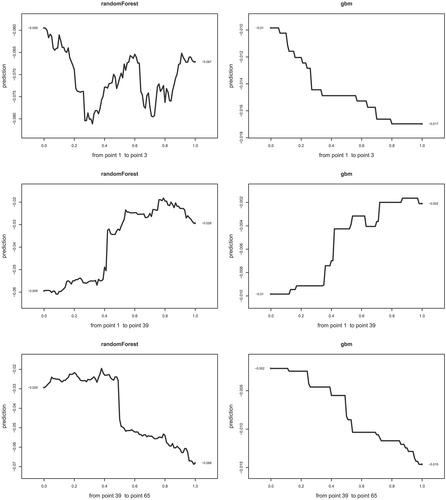
\includegraphics[width=15cm]{Fig13.png}
		}
		\subfigure[Replot]{
			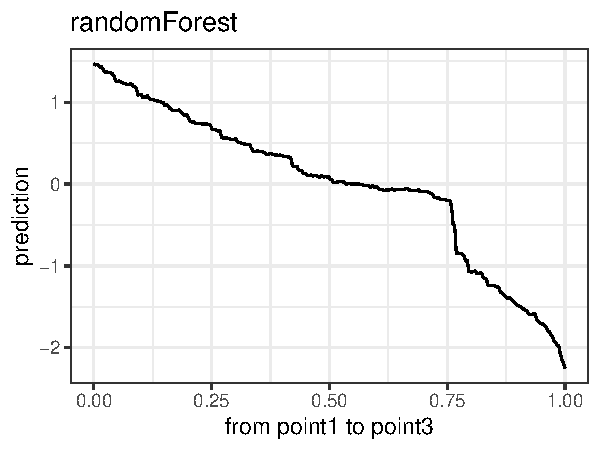
\includegraphics[width=7.7cm]{fig131.pdf}
		}
		\subfigure[Replot]{
			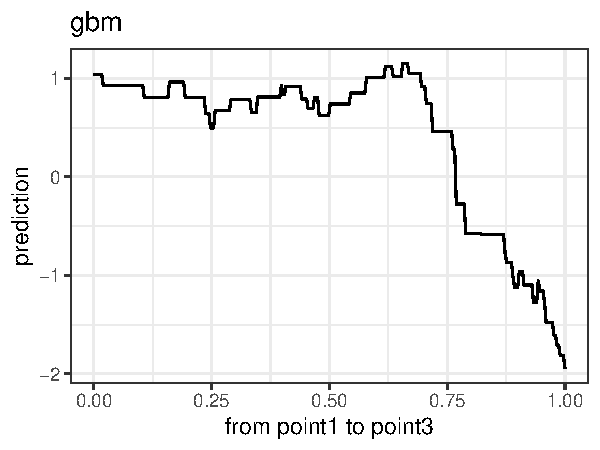
\includegraphics[width=7.7cm]{fig132.pdf}
		}
		\caption{Interpolation between pairs of points in supernova data. Left side is randomForest, right side is gbm.}
		\label{fig13}
\end{figure}

\section{A Comparison Checklist}

Prediction和estimation不一样,尽管这两者经常被混为一谈。这篇文章的大部分是在关注差异。作为对过去的总结以及进行更广泛讨论的出发点,本节列出了一些重要的区别以及它们在统计实践方面的含义。

The new millennium got off to a strong start on the virtues of prediction with \cite{breiman2001statistical} Statistical Science publication, "Statistical Modeling: The Two Cultures." An energetic and passionate argument for the "algorithmic culture"—what I have been calling the pure prediction algorithms—in this work Leo excoriated the "data modeling culture" (i.e., traditional methods) as of limited utility in the dawning world of Big Data. Professor David Cox, the lead discussant, countered with a characteristically balanced defense of mainstream statistics, not rejecting prediction algorithms but pointing out their limitations. I was the second discussant, somewhat skeptical of Leo's claims (which were effusive toward random forests, at that time new) but also somewhat impressed. 

事实证明,Breiman比我更有先见之明:在21世纪,纯预测算法抓住了统计学的聚光灯,在很大程度上沿着Leo提出的思路不断发展。本文可以认为是我在继续努力回答预测算法如何与传统回归推断相关联的问题(\textcolor{blue}{The present paper can be thought of as a continued effort on my part to answer the question of how prediction algorithms relate to traditional regression inference})。

表(\ref{table5})列出了区分传统回归方法和纯预测算法的6个标准。

\begin{table}[H]
    \centering
    \caption{A comparison checklist of differences between traditional regression methods and pure prediction algorithms.}
    \label{table5}
    \begin{tabular}{lll}
    \toprule
        &Traditional regressions methods &  Pure prediction algorithms \\
    \midrule
        1. & Surface plus noise models (continuous, smooth) & Direct prediction (possibly discrete, jagged) \\
        2. & Scientific truth (long‐term) & Empirical prediction accuracy (possibly short‐term) \\ 
        3. & Parametric modeling (causality) & Nonparametric (black box) \\
        4. & Parsimonious modeling (researchers choose covariates) & Anti‐parsimony (algorithm chooses predictors) \\ 
        5. & $\bold{x}_{p\times n}$: with $p \ll n$  (homogeneous data) &  $p \gg n$ , both possibly enormous (mixed data) \\ 
        6. & Theory of optimal inference (mle, Neyman-Pearson) & Training/test paradigm (Common Task Framework) \\ 
    \bottomrule
    \end{tabular}
\end{table}

\textbf{标准1}:surface plus noise模型在传统回归方法中普遍存在,以至于在纯预测世界中它们的缺失是令人不安的。random forest,gbm或它们的同类都不需要surface或者noise这样的输入,在易于使用方面是一个巨大的优势。此外,如果没有模型也就无法使用错误的模型。

prostate cancer的临床医生肯定会对有效的预测感兴趣,但研究科学家更感兴趣的是疾病的病因,这就是传统统计方法发挥作用的地方。纯预测算法不考虑surface会造成很多不好的后果,其中受到破坏的就是平滑度(smoothness)。预测算法的主要目的是达到非常好的预测效果,大多集中在离散的目标空间中,如亚马逊推荐、翻译程序、驾驶方向等,这些都和平滑度无关。将它们用于科学研究的愿望可能会加速开发出更平滑、更合理的算法。

\textbf{标准2}:遵循着200年的科学道路,传统的回归方法旨在从噪声数据中提取潜在的真理:虽然不是永恒的真理,但至少是一些超越当前经验的启示。

如果不需要surface plus noise机制,在预测方面,探索科学真相的重要性就会减弱,可能不存在任何潜在的真相。预测方法可以适应短暂的关系,这些关系只需要下一次更新之前保持有效即可。引用Breiman的话,"The theory in this field shifts focus from data models to the properties of algorithms",也就是从物理世界转移到计算机。预测算法的研究确实主要集中在算法的计算特性上,特别是当$n$和$p$变得巨大时它们表现如何,而较少关注它们与数据生成模型之间的关系。

\textbf{标准3}:参数化建模在传统推断方法中扮演着中心角色,而预测算法是非参数化的(非参数可能涉及大量的调整参数,在深度学习中有数百万个这样的参数,所有这些参数都与算法有关,而与数据的生成无关)。参数模型的背后通常隐藏着一些因果关系。在第2节图(\ref{fig1})的例子中,我们可能认为增加药物cholostyramine的摄入会导致胆固醇呈s型下降,即使严格的因果关系是我们难以摸透的。

放弃数学模型就等于放弃了解自然这一历史性的科学目标。Breiman直言不讳地陈述道:"Data models are rarely used in this community [the algorithmic culture]. The approach is that nature produces data in a black box whose insides are complex, mysterious, and at least partly unknowable." black-box方法在科学上有一种反智力(anti-intellectual)的感觉,但从另一方面看,如果预测是唯一的目标,科学理解可能就无关紧要了。

\textbf{标准4}:表(\ref{table1})中的11个新生儿预测变量是从最初的81个预测变量中筛选出来的。精简建模(Parsimonious modeling)是传统方法的一个特征,对于estimation尤其是attribution来说是至关重要的,因为在通常情况下,发现的能力会随着预测变量的增加而减弱。

纯预测算法是反简约的(Anti‐parsimony),算法可以创造出高度交互的新特征,例如random forest的树变量。Breiman说道:“预测变量越多,信息就越多”,这是一个对深度学习时代特别准确的预测。

但是我是持怀疑态度的。我对Breiman的论文的评论是这样开头的:乍一看,Leo Breiman的这篇令人振奋的论文似乎是在反对parsimony和scientific insight,并支持使用带有许多旋塞(可以理解为许多调整参数)的black boxes。再一看,它仍然是这样,但这篇论文很有启发性···(\textcolor{blue}{At first glance Leo Breiman's stimulating paper looks like an argument against parsimony and scientific insight, and in favor of black boxes with lots of knobs to twiddle. At second glance it still looks that way, but the paper is stimulating...})。创造出的特征(coined features)似乎属于弱学习者类型,可能比表(\ref{table1})中假定的强学习者更短暂。

在第6节提到,如果预测算法是通过一群弱学习者的巧妙组合而起作用的,那么它们在prediction方面比estimation (特别是attribution)更有用。短期科学(Short-term science)是一个矛盾词。将预测算法用在科学发现中将取决于其长期有效性的证明(\textcolor{blue}{The use of prediction algorithms for scientific discovery will depend on demonstrations of their longer-term validity})。

\textbf{标准5}:传统的应用要求$n\times p$数据矩阵$\bold{x}$的$n$充分大于$p$,也许是$n > 5\cdot p$,这样的数据被称为tall data。neonate data中$n=812$、$p=11$完全符合tall data。第7节的supernova data中$n=75$、$p=25$就没有完美符合tall data。而纯预测算法允许甚至鼓励wide data,$p \gg n$。prostate cancer microarray的研究数据明显属于wide data,其中$n=102$、$p=6033$。即使我们一开始是对tall data进行分析,如cholostyramine的例子,预测算法会创造一些新的特征来扩大原始数据。

预测算法如何在$p \gg n$的情况下避免过拟合?有各种各样的答案,但没有一个是完全令人信服的:首先,使用测试集可以保证对误差进行诚实评估;第二,大多数算法在训练阶段会使用交叉验证进行检验;最后,there is an active research area that purports to show a "self-regularizing" property of the algorithms such that even running one of them long past the point where the training data are perfectly fit, as in Figure \ref{fig9} of Section 6, will still produce reasonable predictions.

estimation特别是attribution在同类数据集中效果最好。在一项从特定疾病类别中选择研究对象的随机临床试验中,所收集的数据具有严格的同质性。而预测算法不要求同质性,这一特点可以使其具有更广泛地应用,在结果的generalizability方面是一个优点,但在可解释性方面是一个缺陷。

纯预测算法的scalability使得对于很大的$n$和$p$也可以产生结果,这是一个危险的优点。这导致了人们对更大规模训练集的渴望。巨大的训练集对预测有很好的效果,使任务更有interpolative且更少extrapolative (更像图 \ref{fig5} 和图 \ref{fig6},更不像图 \ref{fig8} 和图 \ref{fig9}),但在attribution方面会造成混淆视听。

传统的回归方法将预测矩阵$\bold{x}$视作一个固定的辅助统计量。这大大简化了参数回归模型的理论;在纯预测的世界中,$\bold{x}$和$\bold{y}$都是随机的,唯一的概率模型是:$\left(x_{i}, y_{i}\right) \stackrel{\text { iid }}{\sim} F$。在纯预测的世界中理论更加困难,encouraging the empirical emphasis discussed in Criterion 6. Bayesian statistics is diminished in the a-probabilistic prediction world, leaving a tacit frequentist basis as the theoretical underpinning.

\textbf{标准6}:传统的统计实践是以一个世纪的理论发展为基础的,极大似然估计和Neyman–Pearson引理是指导应用方法学的最优性准则。在表(\ref{table5})的prediction方面,理论的有效性被经验方法所代替,尤其是对训练集和测试的误差估计方面。

Prediction的优点是无需进行理论建模,但由于缺乏坚实的理论架构,导致了百花齐放:流行的纯预测算法之间是完全不同的。在过去的四分之一个世纪里,先是神经网络,然后是支持向量机,boosting,随机森林,以及以深度学习形式出现的神经网络都处在焦点位置。在缺乏理论指导的情况下,我们或许可以期待更多。

在所谓的"Common Task Framework"中,用各种预测类比赛为算法评分,取代了理论的标准。常见的任务是围绕着一些众所周知的数据集进行预测分析,其中最有名的是Netflix电影推荐数据。这些都不能很好的替代最优预测理论,虽然最优预测理论目前还不存在。

测试集是估计预测误差的可靠工具,但从完整的数据集$\bold{d}$中随机选取测试集可能会削弱推断效果。即使是适度的drift也会大大增加实际的预测误差,如第6节的prostate microarray数据。在某些情况下,除了随机选择法还有一些其他方法,例如early/late division,如图(\ref{fig8})和(\ref{fig9})所示。在第7节的supernova data中,我们的目标是将预测准则应用于距离地球更远的supernovas,因此选择距离地球更远的supernovas作为测试集可能是谨慎的。

在20世纪20年代之前,统计学家并没有真正理解estimation,而在Fisher的工作之后,我们理解了。我们在大规模预测算法方面也处于同样的情况:有很多好的想法和令人兴奋的东西,但没有从原则上理解他们,but progress may be in the air。

\section{Traditional Methods in theWide Data Era}

纯预测算法的成功对传统的理论和实践都产生了激励作用。传统统计的理论在20世纪上半叶形成,主要面向tall data:$n$很小且$p$更小,通常只是$p=1$或$p=2$。不管人们是否喜欢预测算法,部分现代科学已经进入了wide data时代。以下有三个例子。

\subsection{Example 11}

大数据并不是预测算法的唯一标识,计算遗传学的研究也是基于大数据进行的,特别是GWAS (genome-wide association study)的形式,即全基因组关联研究。An impressive example was given by \cite{ikram2010four} in a study concerning the narrowing of blood vessels in the eye.测量了$n=15,358$个人的narrowing,对每个人的基因组进行了评估,大约$p=10^6$个SNPs (single-nucleotide polymorphisms)。这一研究的目的就是发现与narrowing of blood vessels相关的SNPs。

在这样的big data下surface plus noise模型将不再适用。取而代之的是对每个SNP进行单独研究:进行线性回归,计算得到$p$值$p_i$。显著性水平为0.05的Bonferroni threshold为:
\begin{align}
\label{threshold}
	p_i \leq 0.05/10^6
\end{align}

\cite{ikram2010four}在曼哈顿图(Manhattan plot)中展示了他们的结果,纵坐标为$z_i = -\log_{10}(p_i)$,横坐标对应的是在基因组中的位置。阈值(\ref{threshold})对应的$z_i \geq 7.3$,拒绝基因无效的原假设。(由于未能找到原始数据集,下图是使用构造的全基因组数据画的Manhattan plot)
\begin{figure}[H]
		\centering
		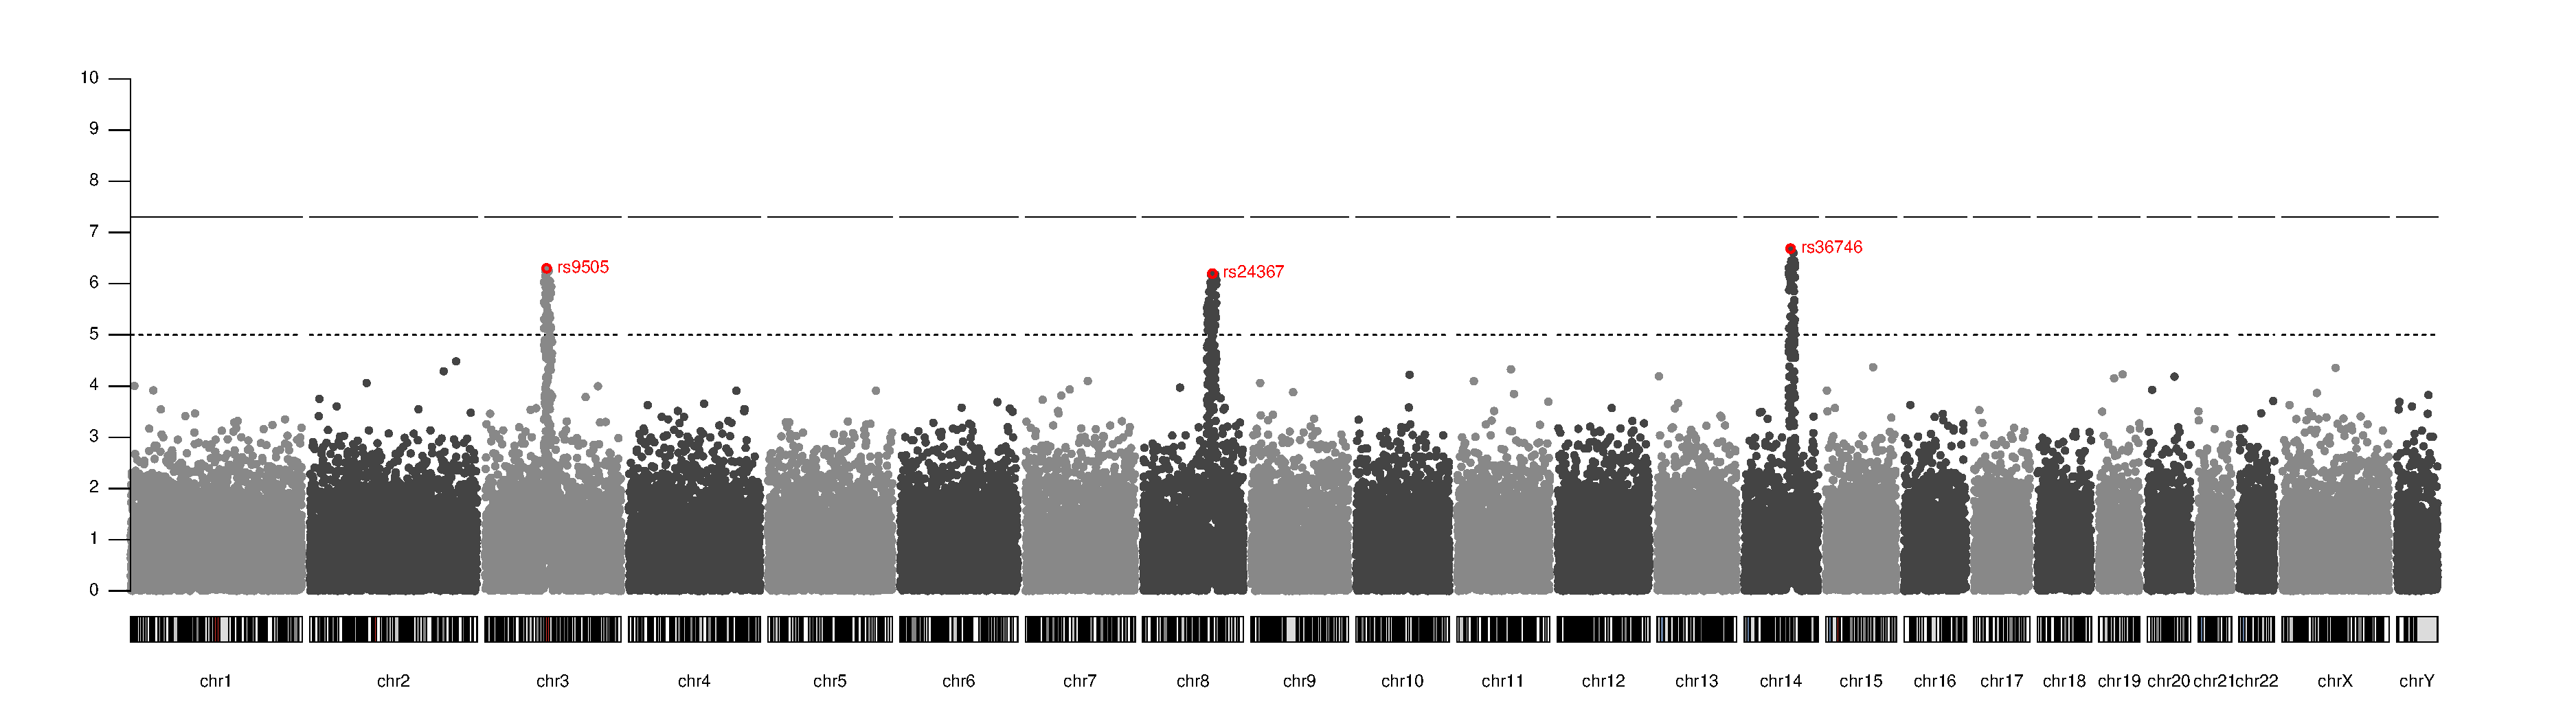
\includegraphics[width=\textwidth]{Manhattan_plot.pdf}
\end{figure}

GWAS没有使用$p = 10^6$个预测变量进行传统的attribution分析,而是令$p=1$进行了$10^6$次attribution分析,然后使用第二层的推断来解释第一层的结果。下一个例子是两层策略更详细的实现。

\subsection{Example 12}

类似于GWAS分析,我们对prostate cancer data进行同样的两层策略实现,对每一个基因进行单独的分析。第$j$个基因的数据可以表示为:
\begin{align}
\bold{d}_{j}=\left\{x_{i j}: i=1,2, \ldots, 102\right\}
\end{align}
其中$i = 1,2, \ldots, 50$是正常控制者,$i = 51,52, \ldots, 102$是癌症患者。

在正态性假设下,我们可以计算统计数据$z_j$:
\begin{align}
z_{j} \sim \mathcal{N}\left(\delta_{j}, 1\right)
\end{align}
其中$\delta_j$表示第$j$个基因的效用大小。

对单个基因本身的推断是直接的。例如:
\begin{align}
p_{j}=2 \Phi\left(-z_{j}\right)
\end{align}
这是用来检验$\delta_j=0$的双边$p$值,然而这忽略了对6033个$p$值的同时解释。与GWAS一样,需要第二层的推断。

贝叶斯分析给效应大小假定了一个先验的密度$g(\delta)$,在$\delta=0$处的概率为$\pi_0$,用来表示无效基因。实际上大多数的基因对prostate cancer都是不起作用的,因此$\pi_0$可以看作接近于1。局部错误发现率$\text{fdr}(z)$,表示给定$z$值$z$的情况下基因是无效基因的概率,根据贝叶斯准则有:
\begin{align}
\text{fdr}(z)=\pi_{0} \phi(z-\delta) / f(z) \doteq \phi(z-\delta) / f(z)
\end{align}
其中$\phi(z)=\exp \left\{-z^{2} / 2\right\} / \sqrt{2 \pi}$,$f(z)$是$z$的边际密度函数:
\begin{align}
f(z)=\int_{-\infty}^{\infty} \phi(z-\delta) g(\delta) d \delta
\end{align}

先验$g(\delta)$大多情况下是未知的。经验贝叶斯分析假设$f(z)$属于某个参数族$f_{\beta}(z)$,通过拟合$f_{\beta}(\cdot)$和数据$\{z_1, z_2, \ldots, z_p \}$得到$\beta$的极大似估计$\hat{\beta}$,从而得到fdr的估计值为:
\begin{align}
\widehat{\text{fdr}}(z)=\phi(z-\delta) / f_{\hat{\beta}}(z)
\end{align}

图(\ref{fig14})中的虚线展示了$\widehat{\text{fdr}}(z)$的结果,其中$f_{\beta}$是通过5阶对数多项式模型得到的:
\begin{align}
\log \left\{f_{\beta}(z)\right\}=\beta_{0}+\sum_{k=1}^{5} \beta_{k} z^{k}
\end{align}
$\widehat{\text{fdr}}(z)$在$|z| < 2$时接近1,对应的基因几乎是无效的。随着$|z|$的增大$\widehat{\text{fdr}}(z)$逐渐降为0,在$z=4$是等于0.129。显著性检验的传统阈值为$\widehat{\text{fdr}}(z) \leq 0.2$,有29个基因满足,表示为图(\ref{fig14})中的三角形。
\begin{figure}[H]
		\centering
		\subfigure[Efron's article]{
			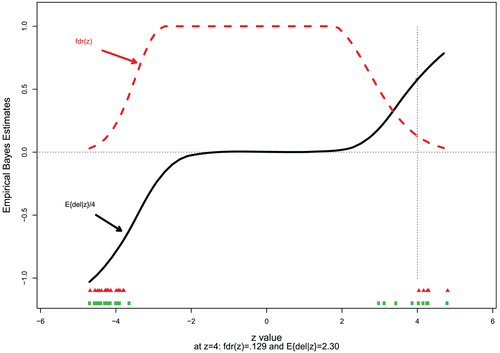
\includegraphics[width=7.7cm]{Fig14.png}
		}
		\subfigure[Replot]{
			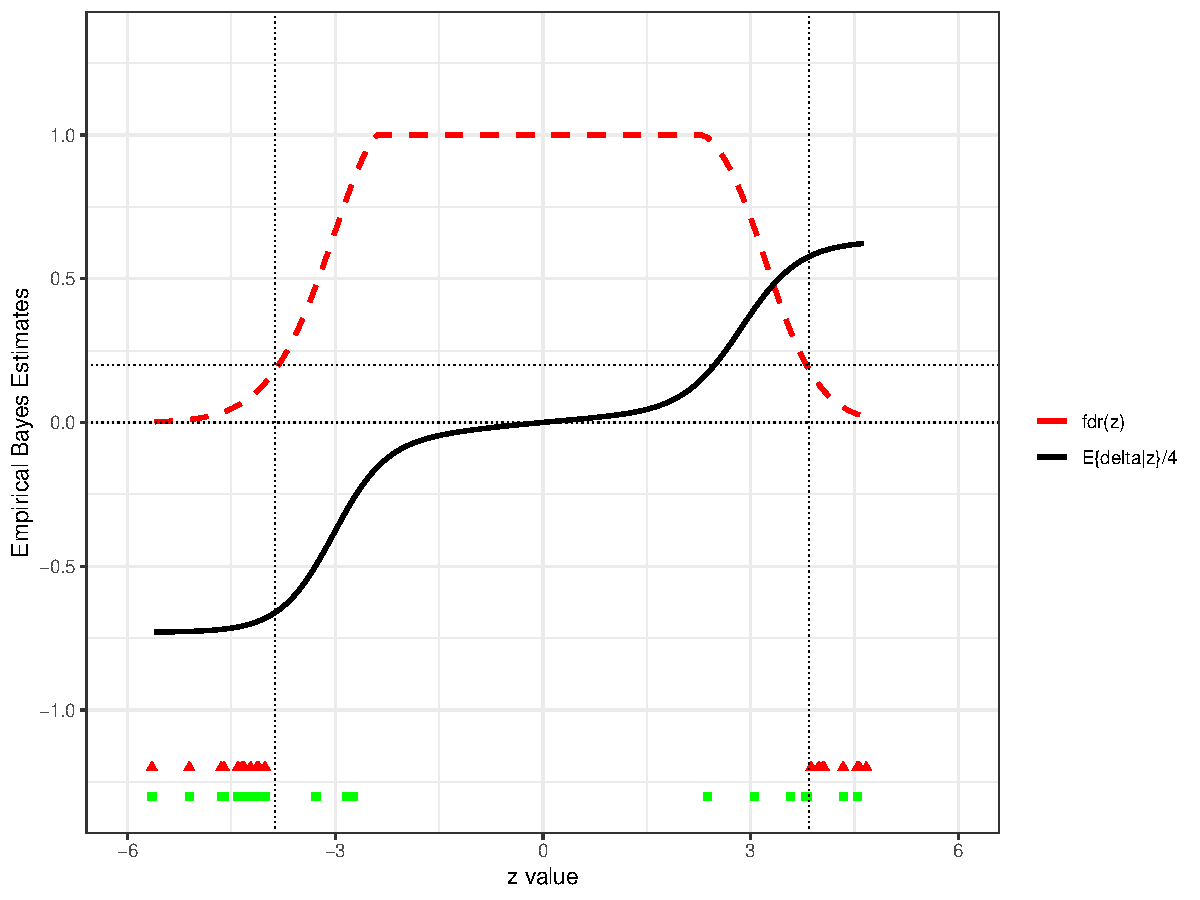
\includegraphics[width=7.7cm]{fig14.pdf}
		}
		\caption{Estimated local false discovery curve $\widehat{\text{fdr}}(z)$ and posterior effect size estimate $\hat{E}\{\delta | z\}$ from empirical Bayes analysis of prostate cancer data (the latter divided by 4 for display purposes). Triangles indicate 29 genes having $\widehat{\text{fdr}}(z) \leq 0.2$; circles are 29 most significant genes from glmnet analysis.}
		\label{fig14}
\end{figure}

我们也可以估计预期的效应大小。\cite{efron2011tweedie}中的Tweedie's formula给出了后验期望的一个简单表达式:
\begin{align}
E\{\delta \mid z\}=z+\frac{d}{d z} \log f(z)
\end{align}
在图(\ref{fig14})中,用$f_{\hat{\beta}}$代替$f$来计算$E\{\delta \mid z\}$,如实线所示。当$|z| \leq 2$是$E\{\delta \mid z\}$接近为0,在$z=4$时上升为2.30。

通过使用一个两层次模型,经验贝叶斯分析将$p=6033$减少到$p=5$。这样就又回到了传统方法的舒适区,可以进行很好的estimation和attribution分析。

稀疏性为wide data的estimation和attribution提供了另一种方法:我们假设$p$个预测变量中的大多数是没有影响的,并集中精力寻找为数不多的重要变量。lasso提供了一个关键的研究方法,通过最小化以下式子来估计$\beta$:
\begin{align}
\frac{1}{n} \sum_{i=1}^{n}\left(y_{i}-x_{i}^{t} \beta\right)^{2}+\lambda\|\beta\|_{1}
\end{align}
其中$\|\beta\|_{1}=\sum_{j=1}^{p}\left|\beta_{j}\right|$。$\lambda$是一个固定的调整参数,$\lambda=0$时$\beta$的估计结果和OLS方法是一样的,$\lambda$取值很大时,只有少数的协变量系数$\hat{\beta}_j$是非零的。lasso方法在$p > n$的情形下也是可行的。图(\ref{fig14})中的方块表示利用lasso方法所筛选的前29个重要的基因。

\subsection{Example 13}

将lasso方法应用到第7节的supernova数据中,其中$\bold{x}$的$n=75$,$p=25$。图(\ref{fig15})显示了在前六步中,非零变量$\hat{\beta}_j$被逐步添加进来的过程。其中预测变量15首先被选取,接下来是变量16,18,22,8和6,在第25步得到完整的$\hat{\beta}$。根据某个精度公式($Cp$值最小)得到第4步为最优的拟合结果,此时只有非零系数15,16,18和22。

\noindent{\textbf{注}:正如前面所述,Rcode中的supernova data数据是人为构造的,因此lasso分析的结果仅供参考。}

\begin{figure}[H]
		\centering
		\subfigure[Efron's article]{
			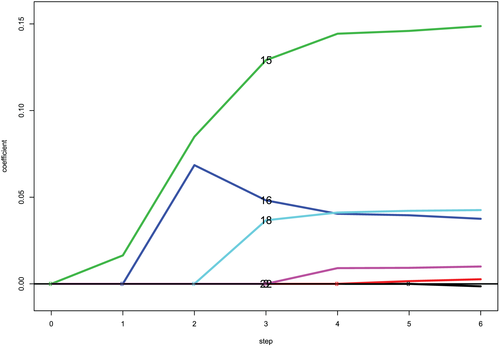
\includegraphics[width=7.7cm]{Fig15.png}
		}
		\subfigure[Replot]{
			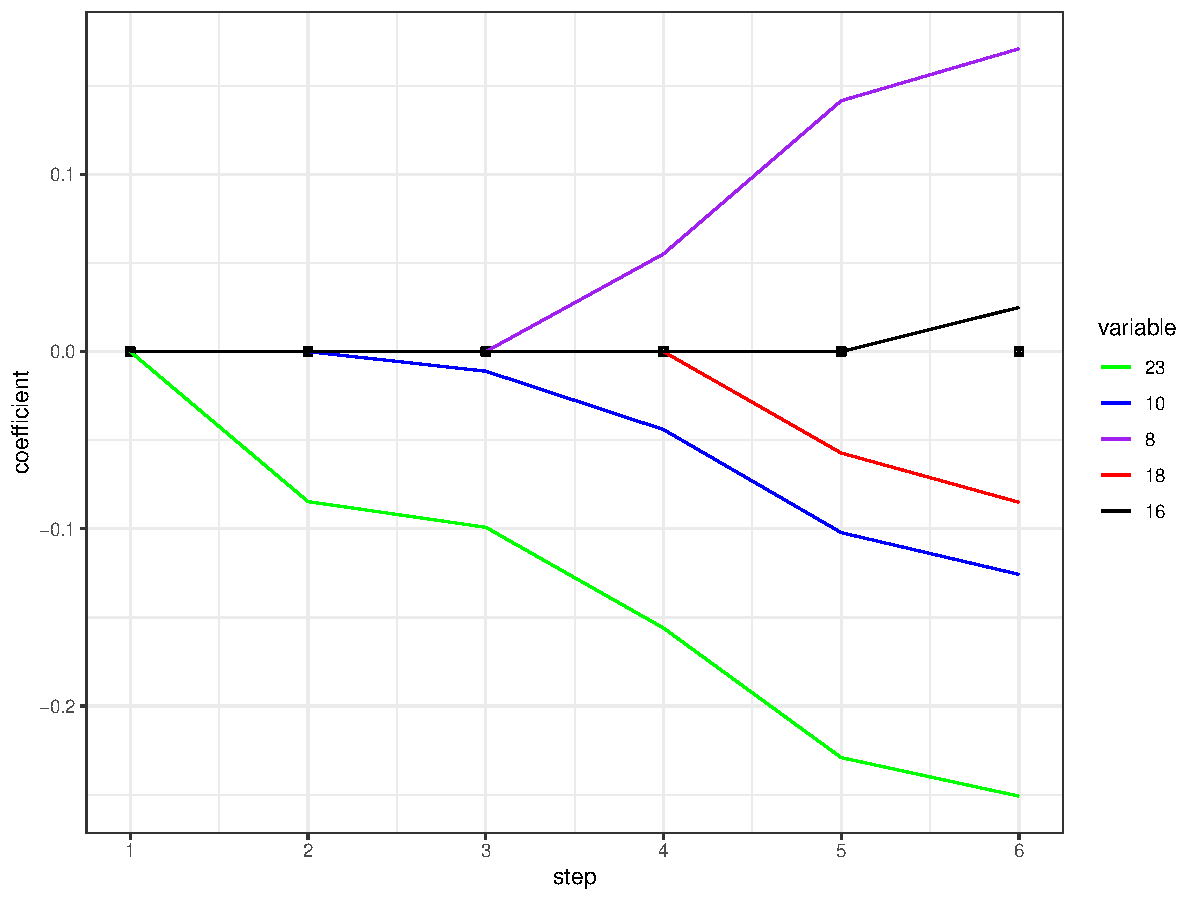
\includegraphics[width=7.7cm]{fig15.pdf}
		}
		\caption{First 6 steps of the lasso algorithm applied to the supernova data; coefficients of various predictors are plotted as a function of step size. Predictor 15 was chosen first, followed by 16, 18, 22, 8, and 6. Stopping at step 4 gives the lowest $Cp$ estimate of estimation error}
		\label{fig15}
\end{figure}

稀疏性和lasso将我们带向与纯预测算法相反的方向。lasso的推断不是结合无数的弱预测变量,而是基于几个最强的解释变量。这很适合attribution,但不太适合prediction。lasso产生了有偏差的$\beta$估计,针对预测方法的批评也适用于此:有偏差的估计还没有建立在坚实的理论基础上(\textcolor{blue}{The criticism leveled at prediction methods also applies here: biased estimation is not yet on a firm theoretical footing})。

\section{Two Hopeful Trends}

\begin{itemize}
	\item Making prediction algorithms better for scientific use
	\begin{itemize}
		\item smoother
		\item more interpretable
		\item less brittle
	\end{itemize}
	\item Making traditional estimation/attribution methods better for large-scale $(n, p)$ problems
	\begin{itemize}
		\item less fussy
		\item more flexible
		\item better scaled
	\end{itemize}
\end{itemize}



\newpage
%\nocite{*}
\bibliography{wpref}

\newpage
\appendix

\end{document}
